\documentclass[]{elsarticle} %review=doublespace preprint=single 5p=2 column
%%% Begin My package additions %%%%%%%%%%%%%%%%%%%
\usepackage[hyphens]{url}
\usepackage{lineno} % add
\providecommand{\tightlist}{%
  \setlength{\itemsep}{0pt}\setlength{\parskip}{0pt}}

\bibliographystyle{elsarticle-harv}
\biboptions{sort&compress} % For natbib
\usepackage{graphicx}
\usepackage{booktabs} % book-quality tables
%% Redefines the elsarticle footer
%\makeatletter
%\def\ps@pprintTitle{%
% \let\@oddhead\@empty
% \let\@evenhead\@empty
% \def\@oddfoot{\it \hfill\today}%
% \let\@evenfoot\@oddfoot}
%\makeatother

% A modified page layout
\textwidth 6.75in
\oddsidemargin -0.15in
\evensidemargin -0.15in
\textheight 9in
\topmargin -0.5in
%%%%%%%%%%%%%%%% end my additions to header

\usepackage[T1]{fontenc}
\usepackage{lmodern}
\usepackage{amssymb,amsmath}
\usepackage{ifxetex,ifluatex}
\usepackage{fixltx2e} % provides \textsubscript
% use upquote if available, for straight quotes in verbatim environments
\IfFileExists{upquote.sty}{\usepackage{upquote}}{}
\ifnum 0\ifxetex 1\fi\ifluatex 1\fi=0 % if pdftex
  \usepackage[utf8]{inputenc}
\else % if luatex or xelatex
  \usepackage{fontspec}
  \ifxetex
    \usepackage{xltxtra,xunicode}
  \fi
  \defaultfontfeatures{Mapping=tex-text,Scale=MatchLowercase}
  \newcommand{\euro}{€}
\fi
% use microtype if available
\IfFileExists{microtype.sty}{\usepackage{microtype}}{}
\usepackage{longtable}
\usepackage{graphicx}
% We will generate all images so they have a width \maxwidth. This means
% that they will get their normal width if they fit onto the page, but
% are scaled down if they would overflow the margins.
\makeatletter
\def\maxwidth{\ifdim\Gin@nat@width>\linewidth\linewidth
\else\Gin@nat@width\fi}
\makeatother
\let\Oldincludegraphics\includegraphics
\renewcommand{\includegraphics}[1]{\Oldincludegraphics[width=\maxwidth]{#1}}
\ifxetex
  \usepackage[setpagesize=false, % page size defined by xetex
              unicode=false, % unicode breaks when used with xetex
              xetex]{hyperref}
\else
  \usepackage[unicode=true]{hyperref}
\fi
\hypersetup{breaklinks=true,
            bookmarks=true,
            pdfauthor={},
            pdftitle={A simplified dynamic bioenergetic model for coral-Symbiodinium symbioses and coral bleaching as an alternate stable state},
            colorlinks=true,
            urlcolor=blue,
            linkcolor=magenta,
            pdfborder={0 0 0}}
\urlstyle{same}  % don't use monospace font for urls
\setlength{\parindent}{0pt}
\setlength{\parskip}{6pt plus 2pt minus 1pt}
\setlength{\emergencystretch}{3em}  % prevent overfull lines
\setcounter{secnumdepth}{0}
% Pandoc toggle for numbering sections (defaults to be off)
\setcounter{secnumdepth}{0}
% Pandoc header


\usepackage[nomarkers]{endfloat}

\begin{document}
\begin{frontmatter}

  \title{A simplified dynamic bioenergetic model for coral-\emph{Symbiodinium}
symbioses and coral bleaching as an alternate stable state}
    \author[University of Hawaii]{Ross Cunning\corref{c1}}
   \ead{ross.cunning@gmail.com} 
   \cortext[c1]{Corresponding Author}
    \author[University of California]{Erik B. Muller}
  
  
    \author[University of Hawaii]{Ruth D. Gates}
  
  
    \author[University of California]{Roger M. Nisbet}
  
  
      \address[University of Hawaii]{Hawaii Institute of Marine Biology, Kaneohe, HI 96744, USA}
    \address[University of California]{Department of Ecology, Evolution, and Marine Biology, Santa Barbara, CA
93106, USA}
  
  \begin{abstract}
  Coral reef ecosystems owe their ecological success--and vulnerability to
  climate change--to the symbiotic metabolism of corals and
  \emph{Symbiodinium} spp. The urgency to understand and predict the
  stability and breakdown of these symbioses (i.e., coral `bleaching')
  demands the development and application of theoretical tools; however,
  the complexity of some approaches may limit their potential application
  and utility. Here, we develop a simplified dynamic bioenergetic model of
  coral-\emph{Symbiodinium} symbioses that demonstrates realistic
  steady-state patterns in coral growth and symbiont abundance across
  gradients of light, nutrients, and feeding. Furthermore, through a
  mechanistic treatment of photo-oxidative stress, the model displays
  dynamic behaviors of bleaching and recovery, and suggests that these
  phenomena represent transitions between alternate stable states. A suite
  of complex responses to multiple, interacting environmental factors
  reproduced by the model suggests it unifyingly captures many important
  attributes of the system; meanwhile, its modular framework and open
  source R code are designed to facilitate expansion and problem-specific
  applications. We see significant potential applications for this
  modeling framework in generating testable hypotheses and predicting
  integrated, mechanistic responses of corals to environmental change.
  \end{abstract}
  
 \end{frontmatter}

\section{Introduction}\label{introduction}

The nutritional exchange between corals and \emph{Symbiodinium} directly
underlies the capacity of corals to build coral reef ecosystems, worth
trillions of US Dollars annually (Costanza, Groot, and Sutton 2014).
However, the complex symbiotic metabolism of corals is vulnerable to
disruption by numerous anthropogenic environmental perturbations,
jeopardizing their future persistence. In order to understand and
predict responses of corals to complex changes in their environment, a
mechanistic understanding of how multiple interacting factors drive the
individual and emergent physiology of both symbiotic partners is
necessary. Such a task is well suited for theoretical modeling
frameworks such as Dynamic Energy Budget (DEB) theory (Kooijman 2010),
although the complexity of such theory makes these efforts inaccessible
to many biologists (Jager, Martin, and Zimmer 2013). In order to bridge
this gap, we present here a simplified dynamic bioenergetic model for
coral-\emph{Symbiodinium} symbioses that aims to mechanistically
integrate the impacts of complex environmental change on the
physiological performance of reef corals, including responses to
environmental stress.

In reef coral symbioses, intracellular \emph{Symbiodinium} translocate
photosynthetically fixed carbon to support coral metabolism, while the
animal host provides access to inorganic nutrients and carbon dioxide
(Muscatine and Porter 1977). Previous application of DEB theory to this
syntrophic system (Muller et al. 2009) demonstrated a stable symbiotic
relationship and qualitatively realistic growth and biomass ratios
across gradients of ambient irradiance, nutrients, and food. This model
assumed that 1) \emph{Symbiodinium} has priority access to fixed carbon
through photosynthesis, 2) the coral animal has priority access to
dissolved nitrogen through contact with seawater, and 3) each partner
shares with the other only what it cannot use for its own growth. In its
simplest form, this principle of sharing the surplus is sufficient to
describe the dynamics of diverse syntrophic organs and organisms (e.g.,
trees, duckweeds, corals), suggesting the mechanism is mathematically
and evolutionarily robust (Nisbet et al., in prep.).

While the formal DEB model of Muller et al. (2009) represents the most
significant theoretical contribution in coral symbiosis research to
date, we aim to strengthen the role of theory and broaden its potential
application in three primary ways:

\begin{enumerate}
\def\labelenumi{\arabic{enumi}.}
\item
  \emph{Develop a module of photooxidative stress.} Of primary interest
  to coral biologists and ecologists is symbiosis dysfunction under
  environmental stress, resulting in coral ``bleaching''--the loss of
  algal symbionts from the association (Jokiel and Coles 1977).
  Photooxidative stress in \emph{Symbiodinium} is considered a primary
  trigger of bleaching in response to high temperature and/or light
  (Weis 2008), and prolonged or severe bleaching can result in
  mortality, though corals sometimes recover their symbionts. Bleaching
  susceptibility, severity, and recovery may be influenced by
  interacting factors such as heterotrophy and nutrient availability
  (Wooldridge 2014b). To simulate these events and interactions, we
  develop a photooxidative stress module linking overreduction of the
  photosynthetic light reactions to downstream impacts of
  photoinhibition and photodamage.
\item
  \emph{Reduce theoretical and mathematical complexity.} Following the
  logic of Jager, Martin, and Zimmer (2013), we exclude certain features
  of formal DEB theory in order to capture behaviors of interest with
  the simplest possible formulation. Here, we present a model without
  reserves, maturity, or reproduction (see Kooijman 2010). This
  formulation restricts the model's scope to the bioenergetics of adult
  corals (i.e., reproduction, larval stages, and metamorphosis are not
  considered), but greatly reduces theoretical complexity and parameter
  numbers, which is advantageous given the relative paucity of data for
  corals. However, our primary motivation for reducing complexity was to
  increase accessibility and applicability for biologists and ecologists
  without requiring significant expertise in DEB theory.
\item
  \emph{Provide well-documented, open-access code.} In order to
  facilitate the continued development and application of theoretical
  modeling tools for coral symbioses, we provide open access to the
  model in the form of detailed, commented code written in the R
  language (R Core Team 2014). With an accessible and modular framework,
  we envision this model as a resource for futher development by the
  scientific community to include additional complexity and
  problem-specific components. We chose the R language, which is freely
  available and in common use by biologists and ecologists, to reach the
  widest possible audience with this work.
\end{enumerate}

With these as our primary motivations, we describe a simplified approach
to dynamic bioenergetic modeling of coral-\emph{Symbiodinium} symbioses
that dynamically integrates the influence of external irradiance,
nutrients, and prey availability on coral growth and symbiosis dynamics
(i.e., symbiont:host biomass ratios), allowing for the possibility of
coral bleaching in the event of photooxidative stress. In the following
sections, we describe and provide rationale for the model structure, and
demonstrate a range of steady state and dynamic behaviors that are
consistent with observed phenomena.

\section{Model description}\label{model-description}

In this dynamical system, both partners acquire and use carbon and
nitrogen to construct biomass: the symbiont fixes carbon through
photosynthesis, and receives nitrogen shared by the host, while the host
acquires nitrogen from the environment and receives carbon shared by the
symbiont. A graphical representation of the model is presented in Fig.
1, and each model flux and parameter is defined in Tables 1 and 2,
respectively. We use C-moles as the unit of biomass for consistency with
the rigorous mass balance of DEB theory: 1 C-mole is equivalent to the
amount of biomass containing 1 mole of carbon atoms. Host biomass
(\(H\)), symbiont biomass (\(S\)), and prey biomass (\(X\)) have fixed,
but different, molar N:C ratios (Table 2). Biomass is produced from
carbon and nitrogen by synthesizing units (SU), which are mathematical
specifications of the formation of a product from two substrates; we use
the parallel complementary formulation of Kooijman (2010) to specify
these fluxes. The two state variables of this system are symbiont
biomass and coral biomass; because resources are acquired proportionally
to surface area, and surface area is proportional to volume (i.e.,
corals are ``V1-morphs'' in DEB terminology (Kooijman 2010)), biomass
increases exponentially during growth (indeed, corals grow exponentially
(Bak 1976)).

Environmental stress is implemented in the form of photooxidative
stress, which is thought to be the primary trigger of coral bleaching
(Lesser 1997; Weis 2008; Wooldridge 2009). To simulate these events, we
model the absorption and quenching of light energy by photochemistry and
non-photochemical quenching, and the phenomenological responses that
occur when these capacities are overwhelmed (i.e., photoinhibition,
photodamage, and symbiont loss). While bleaching in response to high
light alone has been observed experimentally (Schutter et al. 2011;
Downs et al. 2013), mass coral bleaching events occur in response to
high temperature (Hoegh-Guldberg 1999); thus, it is important to justify
our consideration of light as the primary stressor. In reality, light
and temperature interact synergistically (Coles and Jokiel 1978; Jones
et al. 1998), and in fact, any stressor that disrupts the quenching of
light energy may lead to bleaching (Wooldridge 2010; Baker and Cunning
2015). This is because the proximate cause of photo-oxidative stress is
excess excitation energy, but the upstream events that lead to this
situation may be diverse: indeed, elevated temperature may inhibit
Rubisco functioning (Jones et al. 1998) and the repair of the D1 protein
in photosystem II (Warner, Fitt, and Schmidt 1999), which reduces the
capacity of photochemical quenching and leads to an excess of light
energy. In this way, elevated temperature serves to reduce the threshold
above which light stresses the system (Hoegh-Guldberg 1999);
importantly, light is still the proximate stressor. Therefore, we
omitted temperature from the model to maintain a desired level of
simplicity, while still allowing photooxidative stress and bleaching to
be simulated with biological realism in response to light.

Below we describe the formulation of each flux in the model.

Table 1. Model fluxes (mass-specific)

\begin{longtable}[c]{@{}llll@{}}
\toprule
\begin{minipage}[b]{0.10\columnwidth}\raggedright\strut
Symbol
\strut\end{minipage} &
\begin{minipage}[b]{0.48\columnwidth}\raggedright\strut
Description
\strut\end{minipage} &
\begin{minipage}[b]{0.25\columnwidth}\raggedright\strut
Units
\strut\end{minipage} &
\begin{minipage}[b]{0.10\columnwidth}\raggedright\strut
Eq. no.
\strut\end{minipage}\tabularnewline
\midrule
\endhead
\begin{minipage}[t]{0.10\columnwidth}\raggedright\strut
\(j_X\)
\strut\end{minipage} &
\begin{minipage}[t]{0.48\columnwidth}\raggedright\strut
Prey uptake rate
\strut\end{minipage} &
\begin{minipage}[t]{0.25\columnwidth}\raggedright\strut
molX CmolH\textsuperscript{-1} d\textsuperscript{-1}
\strut\end{minipage} &
\begin{minipage}[t]{0.10\columnwidth}\raggedright\strut
3
\strut\end{minipage}\tabularnewline
\begin{minipage}[t]{0.10\columnwidth}\raggedright\strut
\(j_N\)
\strut\end{minipage} &
\begin{minipage}[t]{0.48\columnwidth}\raggedright\strut
Nitrogen uptake rate
\strut\end{minipage} &
\begin{minipage}[t]{0.25\columnwidth}\raggedright\strut
molN CmolH\textsuperscript{-1} d\textsuperscript{-1}
\strut\end{minipage} &
\begin{minipage}[t]{0.10\columnwidth}\raggedright\strut
4
\strut\end{minipage}\tabularnewline
\begin{minipage}[t]{0.10\columnwidth}\raggedright\strut
\(j_{HG}\)
\strut\end{minipage} &
\begin{minipage}[t]{0.48\columnwidth}\raggedright\strut
Host biomass formation rate
\strut\end{minipage} &
\begin{minipage}[t]{0.25\columnwidth}\raggedright\strut
CmolH CmolH\textsuperscript{-1} d\textsuperscript{-1}
\strut\end{minipage} &
\begin{minipage}[t]{0.10\columnwidth}\raggedright\strut
5
\strut\end{minipage}\tabularnewline
\begin{minipage}[t]{0.10\columnwidth}\raggedright\strut
\(r_{NH}\)
\strut\end{minipage} &
\begin{minipage}[t]{0.48\columnwidth}\raggedright\strut
Recycled nitrogen from host turnover
\strut\end{minipage} &
\begin{minipage}[t]{0.25\columnwidth}\raggedright\strut
molN CmolH\textsuperscript{-1} d\textsuperscript{-1}
\strut\end{minipage} &
\begin{minipage}[t]{0.10\columnwidth}\raggedright\strut
6
\strut\end{minipage}\tabularnewline
\begin{minipage}[t]{0.10\columnwidth}\raggedright\strut
\(\rho_N\)
\strut\end{minipage} &
\begin{minipage}[t]{0.48\columnwidth}\raggedright\strut
Nitrogen shared with the symbiont
\strut\end{minipage} &
\begin{minipage}[t]{0.25\columnwidth}\raggedright\strut
molN CmolH\textsuperscript{-1} d\textsuperscript{-1}
\strut\end{minipage} &
\begin{minipage}[t]{0.10\columnwidth}\raggedright\strut
7
\strut\end{minipage}\tabularnewline
\begin{minipage}[t]{0.10\columnwidth}\raggedright\strut
\(j_{eC}\)
\strut\end{minipage} &
\begin{minipage}[t]{0.48\columnwidth}\raggedright\strut
Excess carbon used to activate host CCMs
\strut\end{minipage} &
\begin{minipage}[t]{0.25\columnwidth}\raggedright\strut
molC CmolH\textsuperscript{-1} d\textsuperscript{-1}
\strut\end{minipage} &
\begin{minipage}[t]{0.10\columnwidth}\raggedright\strut
8
\strut\end{minipage}\tabularnewline
\begin{minipage}[t]{0.10\columnwidth}\raggedright\strut
\(j_{CO_2}\)
\strut\end{minipage} &
\begin{minipage}[t]{0.48\columnwidth}\raggedright\strut
CO\textsubscript{2} input to photosynthesis
\strut\end{minipage} &
\begin{minipage}[t]{0.25\columnwidth}\raggedright\strut
molCO\textsubscript{2} CmolH\textsuperscript{-1} d\textsuperscript{-1}
\strut\end{minipage} &
\begin{minipage}[t]{0.10\columnwidth}\raggedright\strut
9
\strut\end{minipage}\tabularnewline
\begin{minipage}[t]{0.10\columnwidth}\raggedright\strut
\(j_L\)
\strut\end{minipage} &
\begin{minipage}[t]{0.48\columnwidth}\raggedright\strut
Light absorption rate
\strut\end{minipage} &
\begin{minipage}[t]{0.25\columnwidth}\raggedright\strut
molph CmolS\textsuperscript{-1} d\textsuperscript{-1}
\strut\end{minipage} &
\begin{minipage}[t]{0.10\columnwidth}\raggedright\strut
11
\strut\end{minipage}\tabularnewline
\begin{minipage}[t]{0.10\columnwidth}\raggedright\strut
\(r_{CH}\)
\strut\end{minipage} &
\begin{minipage}[t]{0.48\columnwidth}\raggedright\strut
Recycled CO\textsubscript{2} from host turnover
\strut\end{minipage} &
\begin{minipage}[t]{0.25\columnwidth}\raggedright\strut
molCO\textsubscript{2} CmolH\textsuperscript{-1} d\textsuperscript{-1}
\strut\end{minipage} &
\begin{minipage}[t]{0.10\columnwidth}\raggedright\strut
12
\strut\end{minipage}\tabularnewline
\begin{minipage}[t]{0.10\columnwidth}\raggedright\strut
\(r_{CS}\)
\strut\end{minipage} &
\begin{minipage}[t]{0.48\columnwidth}\raggedright\strut
Recycled CO\textsubscript{2} from symbiont turnover
\strut\end{minipage} &
\begin{minipage}[t]{0.25\columnwidth}\raggedright\strut
molCO\textsubscript{2} CmolS\textsuperscript{-1} d\textsuperscript{-1}
\strut\end{minipage} &
\begin{minipage}[t]{0.10\columnwidth}\raggedright\strut
13
\strut\end{minipage}\tabularnewline
\begin{minipage}[t]{0.10\columnwidth}\raggedright\strut
\(j_{CP}\)
\strut\end{minipage} &
\begin{minipage}[t]{0.48\columnwidth}\raggedright\strut
Photosynthesis rate
\strut\end{minipage} &
\begin{minipage}[t]{0.25\columnwidth}\raggedright\strut
molC CmolS\textsuperscript{-1} d\textsuperscript{-1}
\strut\end{minipage} &
\begin{minipage}[t]{0.10\columnwidth}\raggedright\strut
14
\strut\end{minipage}\tabularnewline
\begin{minipage}[t]{0.10\columnwidth}\raggedright\strut
\(j_{eL}\)
\strut\end{minipage} &
\begin{minipage}[t]{0.48\columnwidth}\raggedright\strut
Light energy in excess of photochemistry
\strut\end{minipage} &
\begin{minipage}[t]{0.25\columnwidth}\raggedright\strut
molph CmolS\textsuperscript{-1} d\textsuperscript{-1}
\strut\end{minipage} &
\begin{minipage}[t]{0.10\columnwidth}\raggedright\strut
15
\strut\end{minipage}\tabularnewline
\begin{minipage}[t]{0.10\columnwidth}\raggedright\strut
\(j_{NPQ}\)
\strut\end{minipage} &
\begin{minipage}[t]{0.48\columnwidth}\raggedright\strut
Total capacity of NPQ
\strut\end{minipage} &
\begin{minipage}[t]{0.25\columnwidth}\raggedright\strut
molph CmolS\textsuperscript{-1} d\textsuperscript{-1}
\strut\end{minipage} &
\begin{minipage}[t]{0.10\columnwidth}\raggedright\strut
16
\strut\end{minipage}\tabularnewline
\begin{minipage}[t]{0.10\columnwidth}\raggedright\strut
\(c_{ROS}\)
\strut\end{minipage} &
\begin{minipage}[t]{0.48\columnwidth}\raggedright\strut
ROS production proportional to baseline
\strut\end{minipage} &
\begin{minipage}[t]{0.25\columnwidth}\raggedright\strut
--
\strut\end{minipage} &
\begin{minipage}[t]{0.10\columnwidth}\raggedright\strut
17
\strut\end{minipage}\tabularnewline
\begin{minipage}[t]{0.10\columnwidth}\raggedright\strut
\(r_{NS}\)
\strut\end{minipage} &
\begin{minipage}[t]{0.48\columnwidth}\raggedright\strut
Recycled nitrogen from symbiont turnover
\strut\end{minipage} &
\begin{minipage}[t]{0.25\columnwidth}\raggedright\strut
molN CmolS\textsuperscript{-1} d\textsuperscript{-1}
\strut\end{minipage} &
\begin{minipage}[t]{0.10\columnwidth}\raggedright\strut
18
\strut\end{minipage}\tabularnewline
\begin{minipage}[t]{0.10\columnwidth}\raggedright\strut
\(j_{SG}\)
\strut\end{minipage} &
\begin{minipage}[t]{0.48\columnwidth}\raggedright\strut
Symbiont biomass formation rate
\strut\end{minipage} &
\begin{minipage}[t]{0.25\columnwidth}\raggedright\strut
CmolS CmolS\textsuperscript{-1} d\textsuperscript{-1}
\strut\end{minipage} &
\begin{minipage}[t]{0.10\columnwidth}\raggedright\strut
19
\strut\end{minipage}\tabularnewline
\begin{minipage}[t]{0.10\columnwidth}\raggedright\strut
\(\rho_C\)
\strut\end{minipage} &
\begin{minipage}[t]{0.48\columnwidth}\raggedright\strut
Fixed carbon shared with host
\strut\end{minipage} &
\begin{minipage}[t]{0.25\columnwidth}\raggedright\strut
molC CmolS\textsuperscript{-1} d\textsuperscript{-1}
\strut\end{minipage} &
\begin{minipage}[t]{0.10\columnwidth}\raggedright\strut
20
\strut\end{minipage}\tabularnewline
\begin{minipage}[t]{0.10\columnwidth}\raggedright\strut
\(j_{ST}\)
\strut\end{minipage} &
\begin{minipage}[t]{0.48\columnwidth}\raggedright\strut
Symbiont turnover rate
\strut\end{minipage} &
\begin{minipage}[t]{0.25\columnwidth}\raggedright\strut
CmolS CmolS\textsuperscript{-1} d\textsuperscript{-1}
\strut\end{minipage} &
\begin{minipage}[t]{0.10\columnwidth}\raggedright\strut
21
\strut\end{minipage}\tabularnewline
\bottomrule
\end{longtable}

Table 2. Model parameters. Derivations of each parameter value along
with supporting references are provided in the Supplementary
Information.

\begin{longtable}[c]{@{}llll@{}}
\toprule
\begin{minipage}[b]{0.10\columnwidth}\raggedright\strut
Symbol
\strut\end{minipage} &
\begin{minipage}[b]{0.48\columnwidth}\raggedright\strut
Description
\strut\end{minipage} &
\begin{minipage}[b]{0.25\columnwidth}\raggedright\strut
Units
\strut\end{minipage} &
\begin{minipage}[b]{0.10\columnwidth}\raggedright\strut
Value
\strut\end{minipage}\tabularnewline
\midrule
\endhead
\begin{minipage}[t]{0.10\columnwidth}\raggedright\strut
\(n_{NH}\)
\strut\end{minipage} &
\begin{minipage}[t]{0.48\columnwidth}\raggedright\strut
N:C molar ratio in host biomass
\strut\end{minipage} &
\begin{minipage}[t]{0.25\columnwidth}\raggedright\strut
--
\strut\end{minipage} &
\begin{minipage}[t]{0.10\columnwidth}\raggedright\strut
\(0.18\)
\strut\end{minipage}\tabularnewline
\begin{minipage}[t]{0.10\columnwidth}\raggedright\strut
\(n_{NS}\)
\strut\end{minipage} &
\begin{minipage}[t]{0.48\columnwidth}\raggedright\strut
N:C molar ratio in symbiont biomass
\strut\end{minipage} &
\begin{minipage}[t]{0.25\columnwidth}\raggedright\strut
--
\strut\end{minipage} &
\begin{minipage}[t]{0.10\columnwidth}\raggedright\strut
\(0.13\)
\strut\end{minipage}\tabularnewline
\begin{minipage}[t]{0.10\columnwidth}\raggedright\strut
\(n_{NX}\)
\strut\end{minipage} &
\begin{minipage}[t]{0.48\columnwidth}\raggedright\strut
N:C molar ratio in prey biomass
\strut\end{minipage} &
\begin{minipage}[t]{0.25\columnwidth}\raggedright\strut
--
\strut\end{minipage} &
\begin{minipage}[t]{0.10\columnwidth}\raggedright\strut
\(0.2\)
\strut\end{minipage}\tabularnewline
\begin{minipage}[t]{0.10\columnwidth}\raggedright\strut
\(j_{HT}^0\)
\strut\end{minipage} &
\begin{minipage}[t]{0.48\columnwidth}\raggedright\strut
Specific turnover rate of host biomass
\strut\end{minipage} &
\begin{minipage}[t]{0.25\columnwidth}\raggedright\strut
CmolH CmolH\textsuperscript{-1} d\textsuperscript{-1}
\strut\end{minipage} &
\begin{minipage}[t]{0.10\columnwidth}\raggedright\strut
\(0.03\)
\strut\end{minipage}\tabularnewline
\begin{minipage}[t]{0.10\columnwidth}\raggedright\strut
\(j_{ST}^0\)
\strut\end{minipage} &
\begin{minipage}[t]{0.48\columnwidth}\raggedright\strut
Specific turnover rate of symbiont biomass
\strut\end{minipage} &
\begin{minipage}[t]{0.25\columnwidth}\raggedright\strut
CmolS CmolS\textsuperscript{-1} d\textsuperscript{-1}
\strut\end{minipage} &
\begin{minipage}[t]{0.10\columnwidth}\raggedright\strut
\(0.03\)
\strut\end{minipage}\tabularnewline
\begin{minipage}[t]{0.10\columnwidth}\raggedright\strut
\(\sigma_{NH}\)
\strut\end{minipage} &
\begin{minipage}[t]{0.48\columnwidth}\raggedright\strut
Proportion host N-turnover recycled to host
\strut\end{minipage} &
\begin{minipage}[t]{0.25\columnwidth}\raggedright\strut
--
\strut\end{minipage} &
\begin{minipage}[t]{0.10\columnwidth}\raggedright\strut
\(0.9\)
\strut\end{minipage}\tabularnewline
\begin{minipage}[t]{0.10\columnwidth}\raggedright\strut
\(\sigma_{CH}\)
\strut\end{minipage} &
\begin{minipage}[t]{0.48\columnwidth}\raggedright\strut
Proportion host C-turnover recycled to photosynthesis
\strut\end{minipage} &
\begin{minipage}[t]{0.25\columnwidth}\raggedright\strut
--
\strut\end{minipage} &
\begin{minipage}[t]{0.10\columnwidth}\raggedright\strut
\(0.1\)
\strut\end{minipage}\tabularnewline
\begin{minipage}[t]{0.10\columnwidth}\raggedright\strut
\(\sigma_{NS}\)
\strut\end{minipage} &
\begin{minipage}[t]{0.48\columnwidth}\raggedright\strut
Proportion symbiont N-turnover recycled to symbiont
\strut\end{minipage} &
\begin{minipage}[t]{0.25\columnwidth}\raggedright\strut
--
\strut\end{minipage} &
\begin{minipage}[t]{0.10\columnwidth}\raggedright\strut
\(0.9\)
\strut\end{minipage}\tabularnewline
\begin{minipage}[t]{0.10\columnwidth}\raggedright\strut
\(\sigma_{CS}\)
\strut\end{minipage} &
\begin{minipage}[t]{0.48\columnwidth}\raggedright\strut
Proportion symbiont C-turnover recycled to photosynthesis
\strut\end{minipage} &
\begin{minipage}[t]{0.25\columnwidth}\raggedright\strut
--
\strut\end{minipage} &
\begin{minipage}[t]{0.10\columnwidth}\raggedright\strut
\(0.9\)
\strut\end{minipage}\tabularnewline
\begin{minipage}[t]{0.10\columnwidth}\raggedright\strut
\(j_{Xm}\)
\strut\end{minipage} &
\begin{minipage}[t]{0.48\columnwidth}\raggedright\strut
Maximum specific feeding rate of host
\strut\end{minipage} &
\begin{minipage}[t]{0.25\columnwidth}\raggedright\strut
molX CmolH\textsuperscript{-1} d\textsuperscript{-1}
\strut\end{minipage} &
\begin{minipage}[t]{0.10\columnwidth}\raggedright\strut
\(0.13\)
\strut\end{minipage}\tabularnewline
\begin{minipage}[t]{0.10\columnwidth}\raggedright\strut
\(K_X\)
\strut\end{minipage} &
\begin{minipage}[t]{0.48\columnwidth}\raggedright\strut
Half-saturation constant for prey uptake by host
\strut\end{minipage} &
\begin{minipage}[t]{0.25\columnwidth}\raggedright\strut
molX L\textsuperscript{-1}
\strut\end{minipage} &
\begin{minipage}[t]{0.10\columnwidth}\raggedright\strut
\(1.95\times 10^{-5}\)
\strut\end{minipage}\tabularnewline
\begin{minipage}[t]{0.10\columnwidth}\raggedright\strut
\(j_{Nm}\)
\strut\end{minipage} &
\begin{minipage}[t]{0.48\columnwidth}\raggedright\strut
Maximum specific DIN uptake rate by host
\strut\end{minipage} &
\begin{minipage}[t]{0.25\columnwidth}\raggedright\strut
molN CmolH\textsuperscript{-1} d\textsuperscript{-1}
\strut\end{minipage} &
\begin{minipage}[t]{0.10\columnwidth}\raggedright\strut
\(0.035\)
\strut\end{minipage}\tabularnewline
\begin{minipage}[t]{0.10\columnwidth}\raggedright\strut
\(K_N\)
\strut\end{minipage} &
\begin{minipage}[t]{0.48\columnwidth}\raggedright\strut
Half-saturation constant for DIN uptake by host
\strut\end{minipage} &
\begin{minipage}[t]{0.25\columnwidth}\raggedright\strut
molN L\textsuperscript{-1}
\strut\end{minipage} &
\begin{minipage}[t]{0.10\columnwidth}\raggedright\strut
\(1.5\times 10^{-6}\)
\strut\end{minipage}\tabularnewline
\begin{minipage}[t]{0.10\columnwidth}\raggedright\strut
\(k_{CO_2}\)
\strut\end{minipage} &
\begin{minipage}[t]{0.48\columnwidth}\raggedright\strut
Efficacy of CO\textsubscript{2} delivery by host CCMs
\strut\end{minipage} &
\begin{minipage}[t]{0.25\columnwidth}\raggedright\strut
molCO\textsubscript{2} molC\textsuperscript{-1}
\strut\end{minipage} &
\begin{minipage}[t]{0.10\columnwidth}\raggedright\strut
\(10\)
\strut\end{minipage}\tabularnewline
\begin{minipage}[t]{0.10\columnwidth}\raggedright\strut
\(j_{HGm}\)
\strut\end{minipage} &
\begin{minipage}[t]{0.48\columnwidth}\raggedright\strut
Maximum specific growth rate of host
\strut\end{minipage} &
\begin{minipage}[t]{0.25\columnwidth}\raggedright\strut
CmolH CmolH\textsuperscript{-1} d\textsuperscript{-1}
\strut\end{minipage} &
\begin{minipage}[t]{0.10\columnwidth}\raggedright\strut
\(1\)
\strut\end{minipage}\tabularnewline
\begin{minipage}[t]{0.10\columnwidth}\raggedright\strut
\(y_{CL}\)
\strut\end{minipage} &
\begin{minipage}[t]{0.48\columnwidth}\raggedright\strut
Quantum yield of photosynthesis
\strut\end{minipage} &
\begin{minipage}[t]{0.25\columnwidth}\raggedright\strut
molC mol ph\textsuperscript{-1}
\strut\end{minipage} &
\begin{minipage}[t]{0.10\columnwidth}\raggedright\strut
\(0.1\)
\strut\end{minipage}\tabularnewline
\begin{minipage}[t]{0.10\columnwidth}\raggedright\strut
\(\bar{a}^*\)
\strut\end{minipage} &
\begin{minipage}[t]{0.48\columnwidth}\raggedright\strut
Effective light-absorbing cross-section of symbiont
\strut\end{minipage} &
\begin{minipage}[t]{0.25\columnwidth}\raggedright\strut
m\textsuperscript{2} CmolS\textsuperscript{-1}
\strut\end{minipage} &
\begin{minipage}[t]{0.10\columnwidth}\raggedright\strut
\(1.34\)
\strut\end{minipage}\tabularnewline
\begin{minipage}[t]{0.10\columnwidth}\raggedright\strut
\(k_{NPQ}\)
\strut\end{minipage} &
\begin{minipage}[t]{0.48\columnwidth}\raggedright\strut
NPQ capacity of symbiont
\strut\end{minipage} &
\begin{minipage}[t]{0.25\columnwidth}\raggedright\strut
mol ph CmolS\textsuperscript{-1} d\textsuperscript{-1}
\strut\end{minipage} &
\begin{minipage}[t]{0.10\columnwidth}\raggedright\strut
\(112\)
\strut\end{minipage}\tabularnewline
\begin{minipage}[t]{0.10\columnwidth}\raggedright\strut
\(k_{ROS}\)
\strut\end{minipage} &
\begin{minipage}[t]{0.48\columnwidth}\raggedright\strut
Excess photon energy that doubles ROS production, relative to baseline
levels
\strut\end{minipage} &
\begin{minipage}[t]{0.25\columnwidth}\raggedright\strut
mol ph CmolS\textsuperscript{-1} d\textsuperscript{-1}
\strut\end{minipage} &
\begin{minipage}[t]{0.10\columnwidth}\raggedright\strut
\(80\)
\strut\end{minipage}\tabularnewline
\begin{minipage}[t]{0.10\columnwidth}\raggedright\strut
\(j_{CPm}\)
\strut\end{minipage} &
\begin{minipage}[t]{0.48\columnwidth}\raggedright\strut
Maximum specific photosynthesis rate of symbiont
\strut\end{minipage} &
\begin{minipage}[t]{0.25\columnwidth}\raggedright\strut
molC CmolS\textsuperscript{-1} d\textsuperscript{-1}
\strut\end{minipage} &
\begin{minipage}[t]{0.10\columnwidth}\raggedright\strut
\(2.8\)
\strut\end{minipage}\tabularnewline
\begin{minipage}[t]{0.10\columnwidth}\raggedright\strut
\(j_{SGm}\)
\strut\end{minipage} &
\begin{minipage}[t]{0.48\columnwidth}\raggedright\strut
Maximum specific growth rate of symbiont
\strut\end{minipage} &
\begin{minipage}[t]{0.25\columnwidth}\raggedright\strut
CmolS CmolS\textsuperscript{-1} d\textsuperscript{-1}
\strut\end{minipage} &
\begin{minipage}[t]{0.10\columnwidth}\raggedright\strut
\(0.25\)
\strut\end{minipage}\tabularnewline
\begin{minipage}[t]{0.10\columnwidth}\raggedright\strut
\(b\)
\strut\end{minipage} &
\begin{minipage}[t]{0.48\columnwidth}\raggedright\strut
Scaling parameter for strength of bleaching response
\strut\end{minipage} &
\begin{minipage}[t]{0.25\columnwidth}\raggedright\strut
--
\strut\end{minipage} &
\begin{minipage}[t]{0.10\columnwidth}\raggedright\strut
\(5\)
\strut\end{minipage}\tabularnewline
\bottomrule
\end{longtable}

\begin{figure}[htbp]
\centering
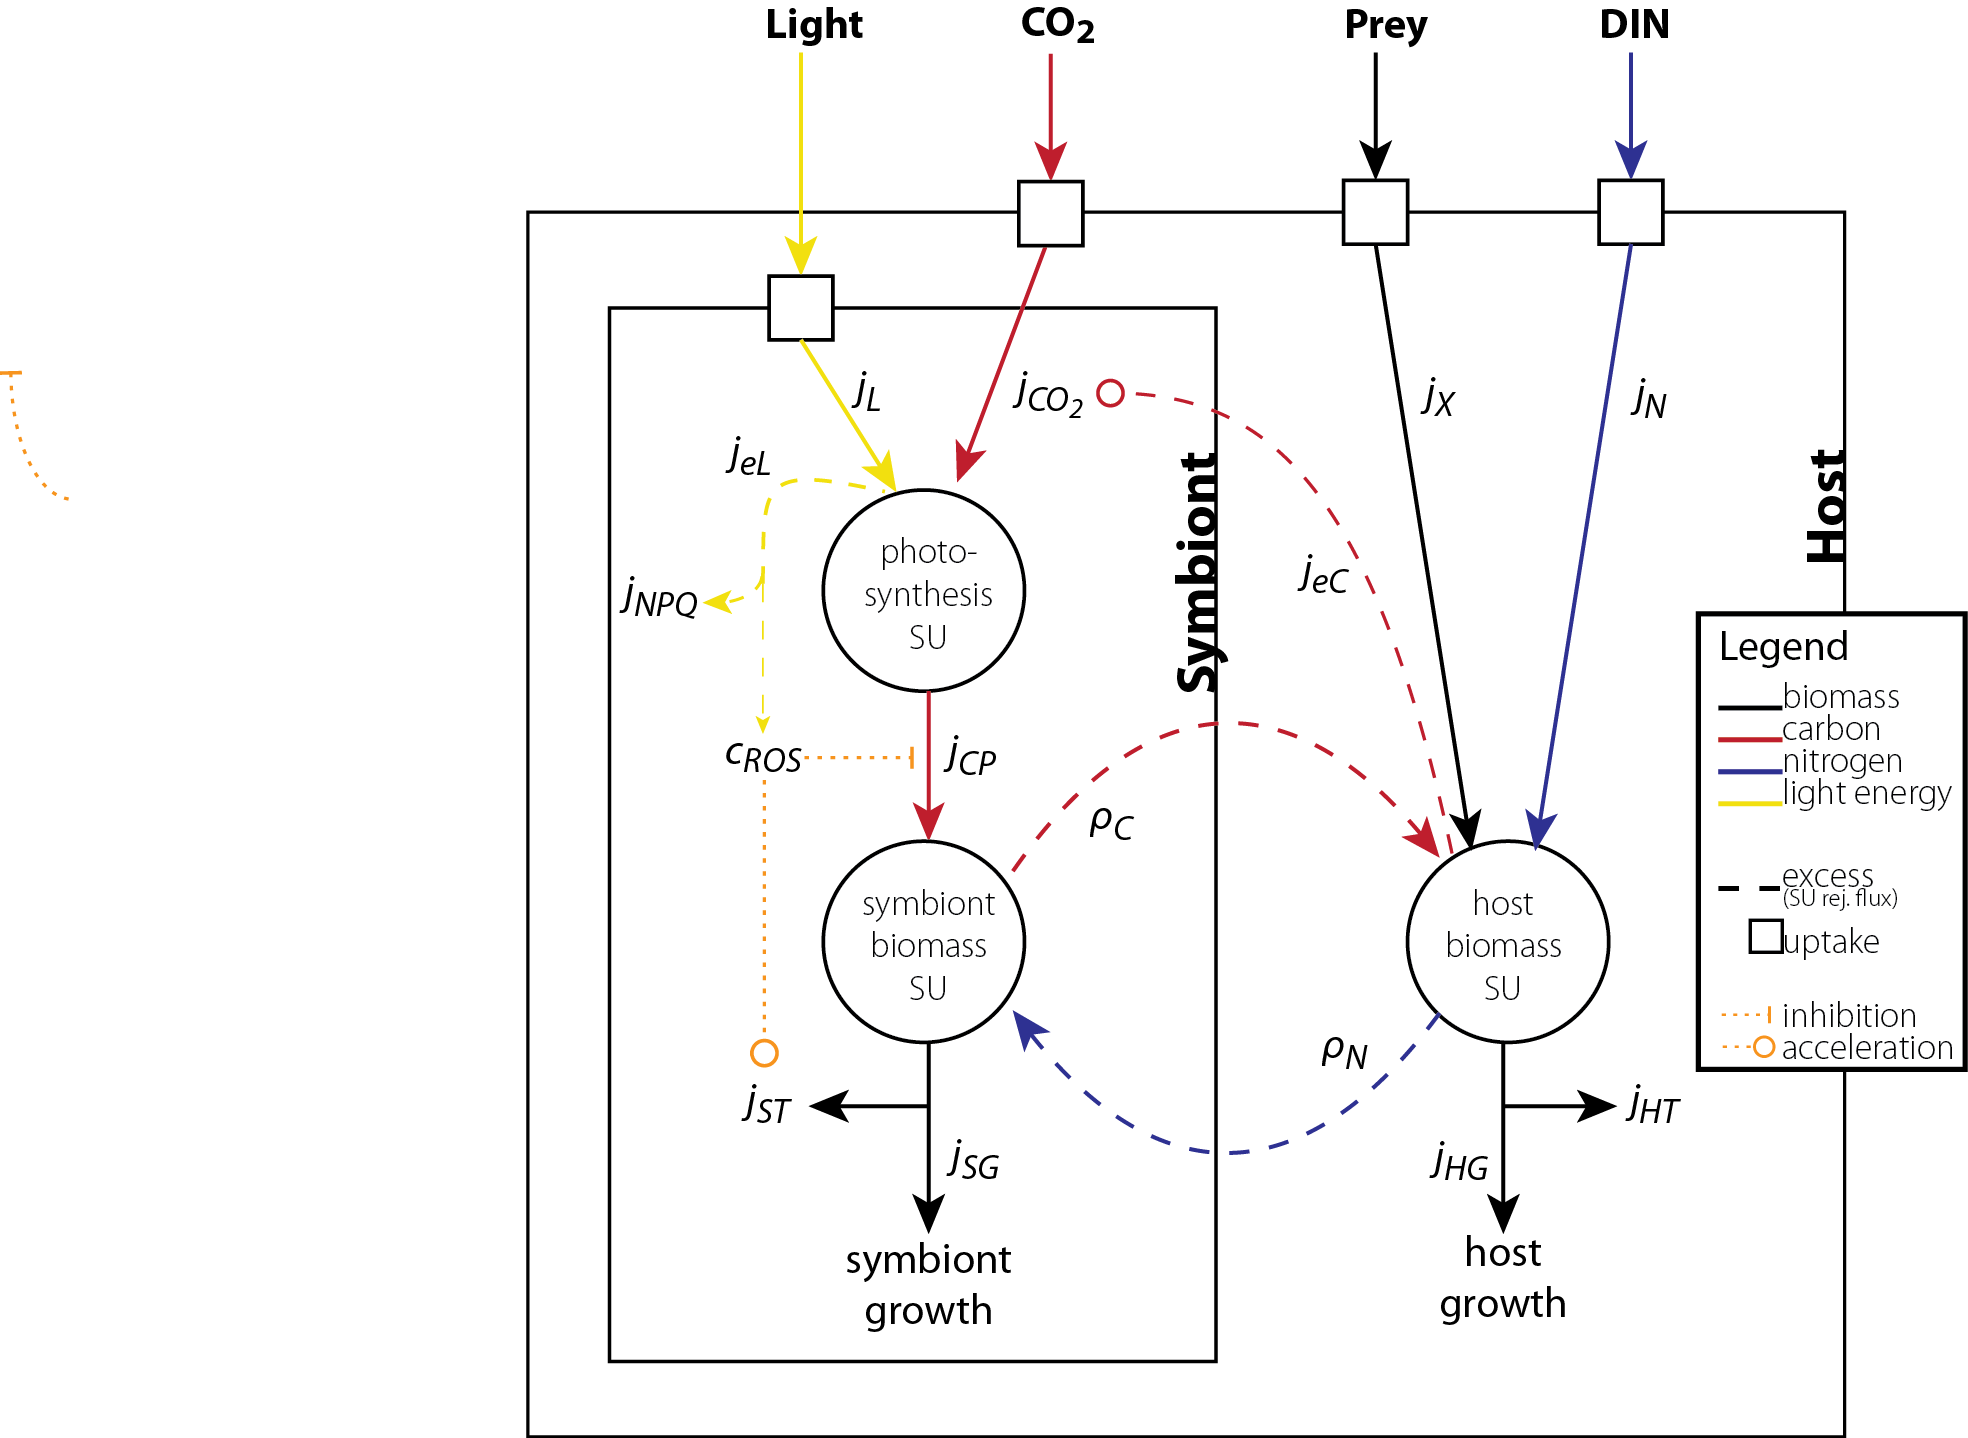
\includegraphics{../img/Fig1.png}
\caption{Graphical representation of coral-algal symbiosis model. Light,
CO\textsubscript{2}, prey, and DIN are acquired from the external
environment proportional to the biomass of the partner indicated by the
black box for uptake. Mass fluxes (see Table 1 for definitions) are
represented by \(j\)'s with subscripts indicating the type of mass, and
in some cases the process (e.g., \(j_{CP}\) is the flux of carbon
produced by photosynthesis), and \(\rho\)'s indicate fluxes that are
shared by one partner with the other. Parallel complementary
synthesizing units (SUs) are represented by large circles, and rejection
fluxes from these SUs are indicated by dashed lines. \(c_{ROS}\) is a
proportional rate that impacts other model fluxes by inhibition or
acceleration; likewise, \(j_{eC}\) accelerates the rate of \(j_{CO_2}\).
Recycled mass fluxes from biomass turnover are not shown for clarity
(but see Table 1 for definitions).}
\end{figure}

\subsection{State equations}\label{state-equations}

The balance equations for symbiont (\(S\)) and host (\(H\)) biomass are
expressed as:

\begin{equation} {dS \over Sdt} = j_{SG} - j_{ST} \end{equation}

\begin{equation} {dH \over Hdt} = j_{HG} - j_{HT}^0 \end{equation}

These are expressed per unit of symbiont and host biomass, respectively.
The specific biomass growth and turnover rates that define these balance
equations are produced by combinations of the individual model fluxes
(see Table 1 for definitions and units), which are each expressed as
mass-specific rates (e.g., per C-mole of symbiont or host biomass per
day). When necessary, conversions between symbiont-mass-specific and
host-mass-specific rates are accomplished by multiplying or dividing by
the symbiont:host biomass ratio.

\subsection{Coral animal fluxes}\label{coral-animal-fluxes}

The coral animal acquires both carbon and nitrogen from feeding on prey
from the environment. Prey acquisition is specified by Michaelis-Menten
kinetics (i.e., a Holling type II function) with a maximum feeding rate
\(j_{Xm}\) and half-saturation constant \(K_X\):

\begin{equation} j_X = {{j_{Xm} \cdot X} \over {X + K_X}} \end{equation}

Additionally, the coral animal acquires nitrogen dissolved in the
surrounding seawater, which is assumed to represent ammonium, the
primary form utilized by corals (Yellowlees, Rees, and Leggat 2008).
This gives the host (rather than the symbiont) priority in nitrogen
utilization; this capacity is supported by experimental evidence (Wang
and Douglas 1998) and is consistent with the physical arrangment of the
partners, where the host is in direct contact with the external
environment. The uptake of nitrogen from the environment is thus
specified by Michaelis-Menten kinetics using a maximum uptake rate
\(j_{Nm}\) and half-saturation constant \(K_N\):

\begin{equation} j_N = {{j_{Nm} \cdot N} \over {N + K_N}} \end{equation}

Coral biomass formation is then specified by a parallel complementary SU
that combines carbon and nitrogen, according to:

\begin{equation} j_{HG} = \bigg({1 \over j_{HGm}} + {1 \over {\rho_C{S \over H} + j_X}} + {1 \over {(j_N + n_{NX}j_X + r_{NH}) / n_{NH}}} - {1 \over {{\rho_C{S \over H} + j_X} + (j_N + n_{NX}j_X + r_{NH}) / n_{NH}}}\bigg)^{-1} \end{equation}

where \(\rho_C\) is fixed carbon shared by the symbiont (see Eq. 20),
and \(r_{NH}\) is recycled nitrogen liberated by host biomass turnover:

\begin{equation} r_{NH}=\sigma_{NH}n_{NH}j_{HT}^0 \end{equation}

The amount of nitrogen input to the coral biomass SU in excess of what
is actually consumed in biomass formation (i.e., surplus nitrogen, or
the rejection flux\footnote{Rejection fluxes must always be positive,
  and hence are specified with the notation \((x)_+\), which means
  \(max(x, 0)\).} of the SU) is then made available to the symbiont:

\begin{equation} \rho_N = (j_N + n_{NX}j_X + r_{NH} - n_{NH}j_{HG})_+ \end{equation}

Due to the inherent inefficiency of the parallel complementary SU
formulation, there is always some nitrogen shared with the symbiont even
when coral biomass formation is strongly nitrogen-limited. Likewise,
there is always a non-zero rejection flux of excess carbon from the
coral biomass SU. Likewise, the carbon rejected from this SU reflects
the amount of excess fixed carbon available to the host that is not used
in biomass formation:

\begin{equation} j_{eC} = (jX + \rho_C{S \over H} - j_{HG})_+ \end{equation}

This flux, \(j_{eC}\), is assumed to be available to the host as a
respiratory substrate to support various energetically-demanding
processes; of particular importance is the host's active carbon
concentrating mechanisms (CCMs) that supply CO\textsubscript{2} for
symbiont photosynthesis (Wooldridge 2013; Hopkinson, Tansik, and Fitt
2015). We therefore specify \(j_{CO_2}\) as the host-mediated delivery
of CO\textsubscript{2} to photosynthesis that encompasses potentially
diverse carbon-concentrating mechanisms (CCMs), including active
transport of bicarbonate, carbonic anhydrase-catalyzed conversion of
bicarbonate to CO\textsubscript{2} to promote diffusion toward the
symbiont (Tansik, Fitt, and Hopkinson 2015), and acidification of the
symbiosome to increase localized CO\textsubscript{2} concentrations
around the symbiont (Barott et al. 2014). Since these active CCMs
require energetic input by the host, we define \(j_{CO_2}\) as
proportional to \(j_{eC}\), assuming that some of this carbon is
respired to energize the CCMs. This formulation means that the symbiont
indirectly ensures its own CO\textsubscript{2} supply by providing fixed
carbon (=energy) to the host (Wooldridge 2013), which establishes a
positive feedback in the model that leads to the existence of multiple
stable states, which we discuss below in the context of coral bleaching.
The parameter \(k_{CO_2}\) scales the efficacy of host CCMs, which
enables the comparison of different rates of CO\textsubscript{2}
delivery that may characterize different coral species (Wooldridge
2014a). The active input of CO\textsubscript{2} to the photosynthesis SU
is therefore specified as:

\begin{equation} j_{CO_2} = k_{CO_2}j_{eC} \end{equation}

\subsection{\texorpdfstring{\emph{Symbiodinium}
fluxes}{Symbiodinium fluxes}}\label{symbiodinium-fluxes}

The symbiont produces fixed carbon through photosynthesis, a process
represented here by a single SU with two substrates: light (photons) and
inorganic carbon (CO\textsubscript{2}). The amount of light absorbed by
the symbiont depends on the scalar irradiance at the site of light
absorption, which is modified substantially relative to external
downwelling irradiance owing to multiple scattering by the coral
skeleton and self-shading by surrounding symbionts (Enríquez, Méndez,
and Iglesias-Prieto 2005; Marcelino et al. 2013). We used data from
Marcelino et al. (2013) to empirically derive an amplification factor,
\(A\), indicating the ratio of internal scalar irradiance to external
downwelling irradiance as a function of symbiont density (S:H biomass),
which is specified as:

\begin{equation} A = 1.26 + 1.39 \cdot \exp(-6.48 \cdot {S \over H}) \end{equation}

This amplification factor is then multiplied by the external downwelling
irradiance \(L\) and the effective light-absorbing surface area of
symbiont biomass \(\bar{a}^*\) to specify the total light absorption:

\begin{equation} j_L =  A \cdot L \cdot \bar{a}^* \end{equation}

CO\textsubscript{2} arrives at the photosynthesis SU from multiple
sources: in addition to the CO\textsubscript{2} actively supplied by the
host through its CCMs (\(j_{CO_2}\); Eq. 9), a fixed proportion of
metabolic CO\textsubscript{2} generated by host biomass turnover is
passively available to the photosynthesis SU, according to:

\begin{equation} r_{CH}=\sigma_{CH}j_{HT}^0 \end{equation}

along with a fixed proportion of CO\textsubscript{2} generated by
symbiont biomass turnover:

\begin{equation} r_{CS}=\sigma_{CS}j_{ST}^0 \end{equation}

Fixed carbon is then produced by the photosynthesis SU according to:

\begin{equation} j_{CP} = \bigg({1 \over j_{CPm}} + {1 \over {y_{CL} j_L }} + {1 \over {(j_{CO_2} + r_{CH}){H \over S} + r_{CS}}} - {1 \over {y_{CL} j_L + (j_{CO_2} + r_{CH}){H \over S} + r_{CS}}}\bigg)^{-1} \cdot c_{ROS}^{-1} \end{equation}

where \(j_{CPm}\) is the maximum specific rate of photosynthesis, and
\(c_{ROS}\) is the relative rate of reactive oxygen species production
(see Eq. 17). Dividing the photosynthetic rate by \(c_{ROS}\) causes a
decline in response to photooxidative stress at high light levels, and
the emergent outcome of this SU formulation demonstrates a classic
photoinhibition response (Fig. S2).

Light energy absorbed in excess of what is used to fix carbon is
specified by the SU rejection flux, according to:

\begin{equation} j_{eL} = (j_L - j_{CP} / y_{CL})_+ \end{equation}

This excess light energy must be quenched by alternative pathways in
order to prevent photooxidative damage (Powles 1984).
\emph{Symbiodinium} utilize a variety of pathways for non-photochemical
quenching (NPQ; Roth 2014), which we collect in a total NPQ capacity
specified as a parameter of the symbiont (\(k_{NPQ}\)). The NPQ flux
\(j_{NPQ}\) is then specified as a single-substrate SU formula with a
maximum of \(k_{NPQ}\):

\begin{equation} j_{NPQ} = \bigg({1 \over k_{NPQ}} + {1 \over j_{eL}}\bigg)^{-1} \end{equation}

If light energy further exceeds the capacity of both photochemistry and
NPQ, then reactive oxygen species (ROS) are produced. We represent this
as a relative quantity \(c_{ROS}\), which takes a value of 1 when all
light energy is quenched by photochemistry and NPQ, and increases as the
amount of excess excitation energy increases, specified as:

\begin{equation} c_{ROS} = 1 + {{(j_{eL} - j_{NPQ})_+} \over k_{ROS}} \end{equation}

where \(k_{ROS}\) is a parameter of the symbiont that determines the
rate of ROS production (specifically, the amount of excess excitation
energy that doubles ROS production relative to baseline levels).
Importantly, \(c_{ROS}\) is specified here not as a function of absolute
external light, but rather the amount of excess light after accounting
for quenching by carbon fixation and NPQ. A direct consequence of this
formulation is that CO\textsubscript{2}-limitation of photosynthesis can
lead to ROS production, an important mechanism (Wooldridge 2009) that
was not captured by previous representations of photooxidative stress
(Eynaud, Nisbet, and Muller 2011).

Carbon fixed by photosynthesis (\(j_{CP}\); Eq. 14) is then combined
with nitrogen shared by the host (\(\rho_N\); Eq. 7) and nitrogen
recycled from symbiont biomass turnover

\begin{equation} r_{NS}=\sigma_{NS}n_{NS}j_{ST}^0 \end{equation}

to build new symbiont biomass, following the SU equation:

\begin{equation} j_{SG} = \bigg({1 \over j_{SGm}} + {1 \over j_{CP}} + {1 \over {(\rho_N{H \over S} + r_{NS}) / n_{NS}}} - {1 \over {j_{CP} + (\rho_N{H \over S} + r_{NS}) / n_{NS}}}\bigg)^{-1} \end{equation}

The rejection flux of carbon from this SU represents the amount of fixed
carbon produced by photosynthesis in excess of what can be used to
produce symbiont biomass; this surplus, \(\rho_C\), is translocated to
the coral host:

\begin{equation} \rho_C = (j_{CP} - j_{SG})_+ \end{equation}

The rejection flux of nitrogen from the symbiont biomass SU is lost to
the environment.

Symbiont biomass turnover includes a component of constant turnover
specified by the parameter \(j_{ST}^0\), representing fixed maintenance
costs, plus a component that scales with the magnitude of ROS
production.

\begin{equation} j_{ST} = j_{ST}^0(1 + b(c_{ROS}-1)) \end{equation}

This second component of symbiont biomass loss represents both
photodamage and/or symbiont expulsion (i.e., bleaching), both of which
occur in response to high levels of ROS production. The parameter \(b\)
is included to scale biomass loss due to bleaching in response to ROS.
(Note that recycling of symbiont biomass turnover (\(rNS\) and \(rCS\))
only occurs based on the maintenance component of turnover (i.e.,
\(j_{ST}^0\)), and not the photodamage/bleaching component, as this loss
represents biomass that is damaged or expelled from the host.)

\subsection{Numerical analysis}\label{numerical-analysis}

The model dynamics are specified by the differential equations (1-2)
that impose biomass balance for host and symbiont and by a set of
coupled non-linear algebraic equations (3-21) that define fluxes.
Several of these fluxes are defined \emph{implicitly}; for example, the
rejection fluxes of carbon and nitrogen from the symbiont and host
biomass SUs, respectively, act as reciprocal input fluxes to the other
SU. Similarly, the photosynthesis SU receives CO\textsubscript{2} at a
rate proportional to the carbon rejection flux from the host biomass SU,
and the rejection flux of excitation energy from the photosynthesis SU
acts to reduce its own production through photoinhibition. Without
further assumptions, however, the dynamical system is not always
unambiguously defined because for some combinations of parameters and
environmental forcing functions the system of algebraic equations has
more than one solution with all fluxes non-negative (see results below).
In such circumstances, the right hand side of the differential equations
(1) and (2) is not uniquely defined even when \(S\) and \(H\) are
specified. We resolved this problem by \emph{defining the dynamical
system} as the limit as a time step \(\Delta t \rightarrow 0\) of a
discretized system corresponding to Euler integration of the
differential equations, with those fluxes that represent flows of
elemental matter implemented by assuming that transfer of material
between components of the system takes one time step. Thus, for example,
CO\textsubscript{2} rejected from the host SU at time \(t\) arrives at
the photosynthesis SU at time \(t + \Delta t\).

Simulations using the discretized scheme were performed using R code
that is available in the data repository accompanying this article:
github.com/jrcunning/Rcoral. By experimentation, we found that a time
step of 0.1 days gave adequate precision for most simulations (including
used to generate Figs. XXX in this paper). For steady state estimations,
simulations were run until the change in specific growth rate of host
and symbiont and the \(S:H\) biomass ratio was less than 1e-5 per time
step. In regions of state space where very slow transient dynamics could
be expected (i.e.~near bifurcation points), sample steady state
calculations were verified using MATHEMATICA code for numerical root
finding (function FindRoot) with the code written independently by a
coauthor without reference to the R code.

To aid in visualizing model results, we calculated values to indicate
the degree to which product formation at an SU was limited by
availability of either of its two substrates using the formula

\begin{equation} \log \bigg({{\min(j_{S1}, j_{Pm})} \over {\min(j_{S2}, j_{Pm})}}\bigg) \end{equation}

where \(j_{S1}\) and \(j_{S2}\) are the specific input fluxes of the two
substrates and \(j_{Pm}\) is the maximum specific product formation
rate, in units of Cmol Cmol\textsuperscript{-1} d\textsuperscript{-1}.

\section{Steady state behavior}\label{steady-state-behavior}

In a constant environment, the system ultimately reaches a steady state
of exponential growth or decline. However, under some conditions, either
of these outcomes may occur depending on initial values of symbiont and
host biomass, indicating the presence of alternate stable states,
corresponding to either positive or negative growth (Fig. 2). The
mechanism that produces these alternate stable states is the positive
feedback between carbon-limitation of the host and
CO\textsubscript{2}-limitation of photosynthesis: if symbiont biomass is
initially very low (i.e., a ``bleached'' coral), the system cannot
escape this positive feedback and cannot grow. However, if symbiont
biomass is initially high (i.e., a ``healthy'' coral), then the system
remains in a nitrogen-limited state with positive growth. For practical
purposes, this section of the manuscript considers only positive growth
steady states under constant environments; the subsequent ``dynamic
behavior'' section explores how changing environments may cause the
system to switch between alternate stable states, which we interpret in
the context of coral bleaching.

\begin{figure}[htbp]
\centering
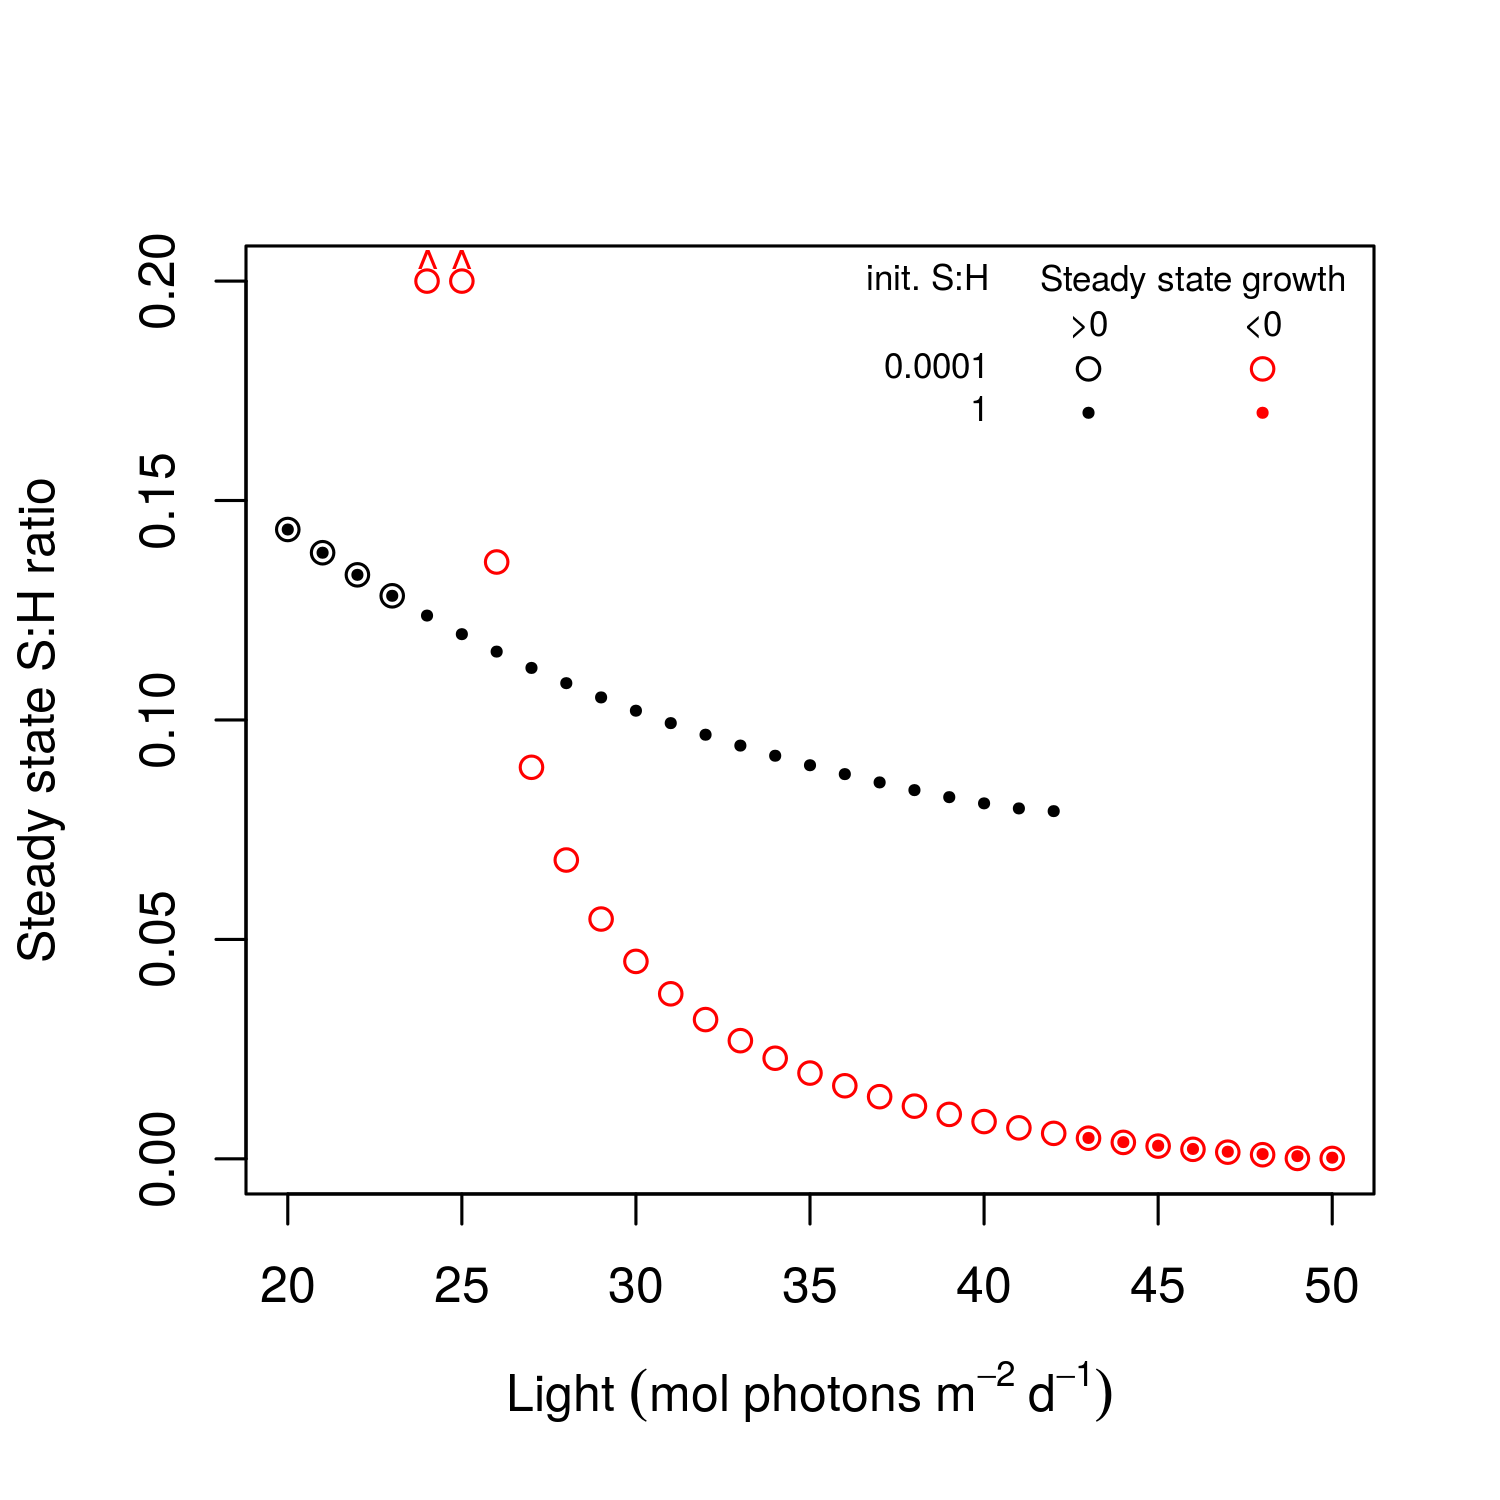
\includegraphics{../img/Fig2.png}
\caption{Alternate stable states}
\end{figure}

To analyze positive-growth steady state behavior, we ran the model to
steady state across gradients of external irradiance and nutrients (Fig.
3), which revealed patterns consistent with observed phenomena in
corals. Predicted growth rates are low at low light and DIN
(\textasciitilde{}0.01 d\textsuperscript{-1}), and begin increasing as
both of these factors increase (Fig. 3A). Low light limits
photosynthetic rates, resulting in less fixed carbon shared with the
host and an associated increase in the symbiont to host biomass ratio
(Fig. 3B). In agreement with this trend are many observations of
negative correlation between irradiance and symbiont density (Stimson
1997; Brown et al. 1999; Fitt et al. 2000; Titlyanov et al. 2001). As
higher light alleviates light-limitation of photosynthesis, host growth
becomes less carbon-limited.

\begin{figure}[htbp]
\centering
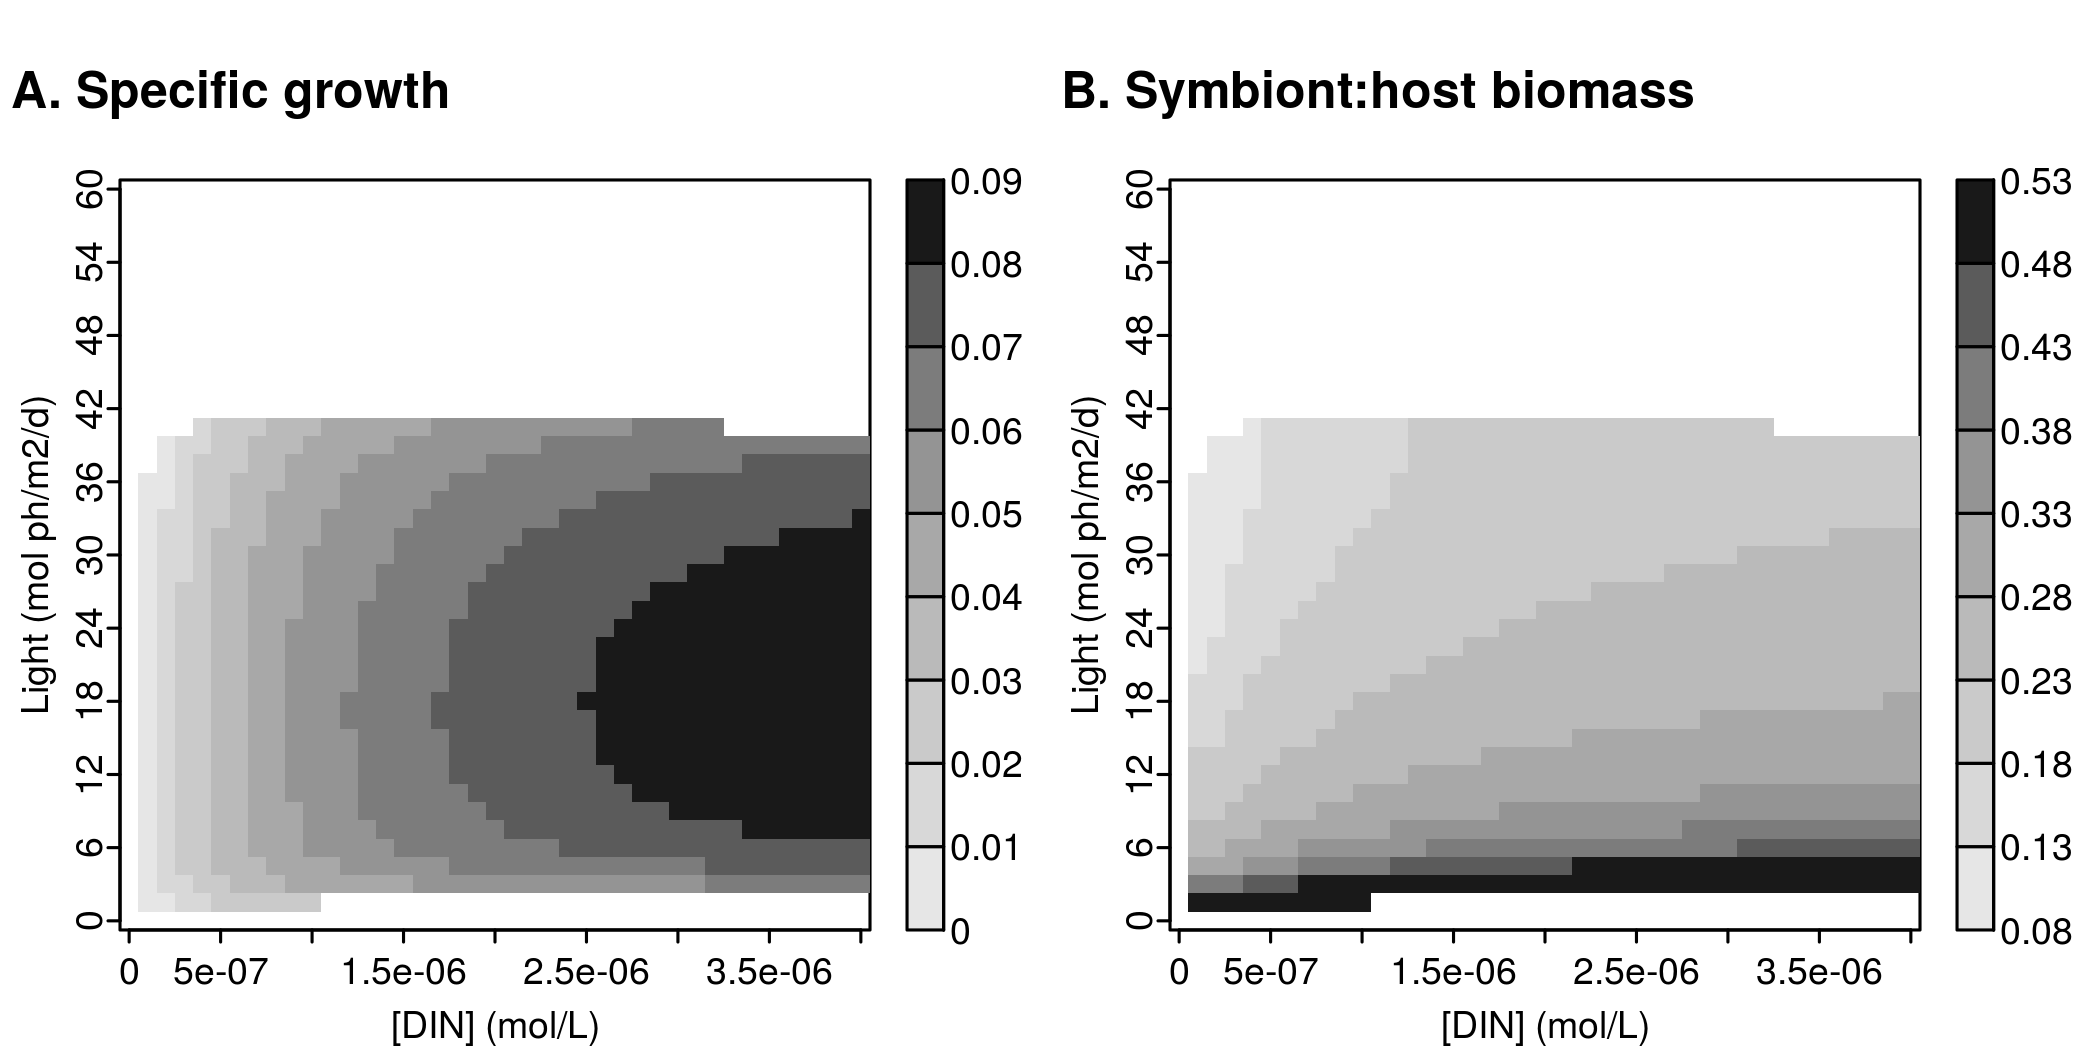
\includegraphics{../img/Fig3.png}
\caption{Steady state values of \textbf{A)} specific growth (Cmol
Cmol\textsuperscript{-1} d\textsuperscript{-1}), \textbf{B)} the
symbiont to host biomass ratio (CmolS CmolH\textsuperscript{-1}),
\textbf{C)} relative C- or N-limitation of host biomass formation, and
\textbf{D)} relative CO\textsubscript{2}- or light-limitation of
symbiont photosynthesis, across gradients of external irradiance and
dissolved inorganic nitrogen. Note that typical conditions for reefs are
\textasciitilde{}1e-7 M DIN and 10-20 mol photons m\textsuperscript{-2}
d\textsuperscript{-1}. Simulations for each combination of light and
nutrients (41 points along each axis) were run for 100 days with a time
step of 1 day. Negative steady state growth rates, and corresponding S:H
ratios, were set to zero.}
\end{figure}

Similarly, increasing DIN alleviates nitrogen-limitation (Fig. 3A).
Increased growth at higher DIN is predicted by the DEB model of Muller
et al. (2009), and has also been observed experimentally (Muller-Parker
et al. 1994; Tanaka et al. 2007; Tanaka et al. 2013). However, DIN
elevation beyond a certain point (e.g., \textasciitilde{}3-4 µM in these
simulations) has little effect on growth as carbon becomes limiting.
Very high nutrient levels may even reduce growth (Shantz, Lemoine, and
Burkepile 2015), although these impacts are not likely to occur within
the range of concentrations considered here (\textless{}4 µM)
(Ferrier-Pagès et al. 2000). In addition to increasing growth, DIN also
increases the symbiont to host biomass ratio (Fig. 3B), a phenomenon
also observed in reef corals (Marubini and Davies 1996). At low DIN and
intermediate light, more typical of coral reef environments, symbiont to
host biomass ratios are around \textasciitilde{}0.06-0.21, which is
consistent with values reported in the literature (Muscatine, R
McCloskey, and E Marian 1981; Edmunds et al. 2011; Hawkins et al. 2016).

The maximum predicted growth rates of \textasciitilde{}0.1
d\textsuperscript{-1}, occurring between \textasciitilde{}10-25 mol
photons m\textsuperscript{-2} s\textsuperscript{-1} light and
\textasciitilde{}4 µM DIN (Fig. 3A), are comparable to the rate of 0.07
d\textsuperscript{-1} measured by Tanaka et al. (2007) under similar
N-enriched conditions. Predicted growth rates under conditions more
typical of reef environments (\textless{}0.5 µM DIN) are
\textasciitilde{}0.01-0.03 d\textsuperscript{-1}. Observed specific
growth rates, which are typically based on skeletal mass, fall near or
below 0.01 d\textsuperscript{-1} (Osinga et al. 2011; Osinga et al.
2012), though values as high as 0.025 d\textsuperscript{-1} have been
reported (Schutter et al. 2010). It is not surprising that predicted
growth rates are slightly higher than most observations, as the model
does not account for external ecological factors that may reduce growth,
such as competition, predation, and bioerosion. Furthermore, the model
does not explicitly account for skeletal formation, which may not always
correlate with biomass growth, potentially due to differential
substrate-limitation (Anthony 2002). Nevertheless, when growth of coral
tissue biomass has been directly measured over short periods, values are
consistent with model predictions (e.g., 0.07 d\textsuperscript{-1} in
Tanaka et al. (2007)), and similar rates (0.04 d\textsuperscript{-1})
have been measured in \emph{Aiptasia diaphana}, a non-calcifying
symbiotic anemone (Armoza-Zvuloni et al. 2014).

As irradiance continues to increase above \textasciitilde{}25 mol
photons m\textsuperscript{-2} d\textsuperscript{-1}, growth rates
decline until positive growth ceases above \textasciitilde{}40 µmol
photons m\textsuperscript{-2} d\textsuperscript{-1} (Fig. 3A). The
mechanism underlying this decline is the increase in light energy beyond
the capacities of photosynthesis and non-photochemical quenching: excess
excitation energy generates reactive oxygen species (ROS) (Weis 2008;
Roth 2014), which, in this model, have the phenomenological consequences
of reducing the photosynthetic rate (representing photoinhibition) and
increasing symbiont biomass loss (representing photodamage and/or
symbiont expulsion) (see Eynaud, Nisbet, and Muller 2011). Together,
these impacts reduce the symbiont to host biomass ratio (Fig. 3B), as
occurs during coral bleaching. This reduction in symbionts consequently
reduces the flux of fixed carbon to the host, resulting in increasing
carbon-limitation (Fig. 3B) and eventual cessation of growth (Fig. 3A).

The incorporation of photooxidative stress in the model sets an upper
limit to the amount of light at which a stable symbiotic interaction can
be maintained, but even below this threshold of breakdown, negative
effects of high light reduce steady state growth and symbiont:host
biomass (Fig. 3). This gradual decline is consistent with experimental
results showing that high light levels decrease growth (Schutter et al.
2011), and field studies documenting optimum growth rates at
intermediate depths (Baker and Weber 1975; Huston 1985). By
incorporating these impacts of light stress, the model predicts greater,
and more realistic, variation in state variables across light gradients
than was predicted by the model of Muller et al. (2009), which did not
include photoinhibition and photodamage. It is important to recognize
that the boundary set by photooxidative stress on a stable symbiosis
under steady state conditions (Fig. 3) may be temporarily crossed by a
dynamic system, which may experience a period of symbiont loss
(bleaching) and reduced growth, after which a return to benign
conditions may restore symbiont biomass and positive growth. To explore
this further and illustrate the behavior of the model in more detail, we
evaluate a number of dynamic simulations below (see ``Dynamic
behavior'').

\section{Sensitivity analysis}\label{sensitivity-analysis}

The values used for each parameter in the model (Table 2) are derived
from relevant literature; these derivations are described in the
Supplementary Information. Here we evaluate the sensitivity of the model
to changes in these parameter values, which also serves to demonstrate
the behavior of the dynamical system. We measured fractional change in
steady state values in response to fractional changes in parameter
values, relative to their default values, under environmental conditions
typical of coral reefs.

\begin{figure}[htbp]
\centering
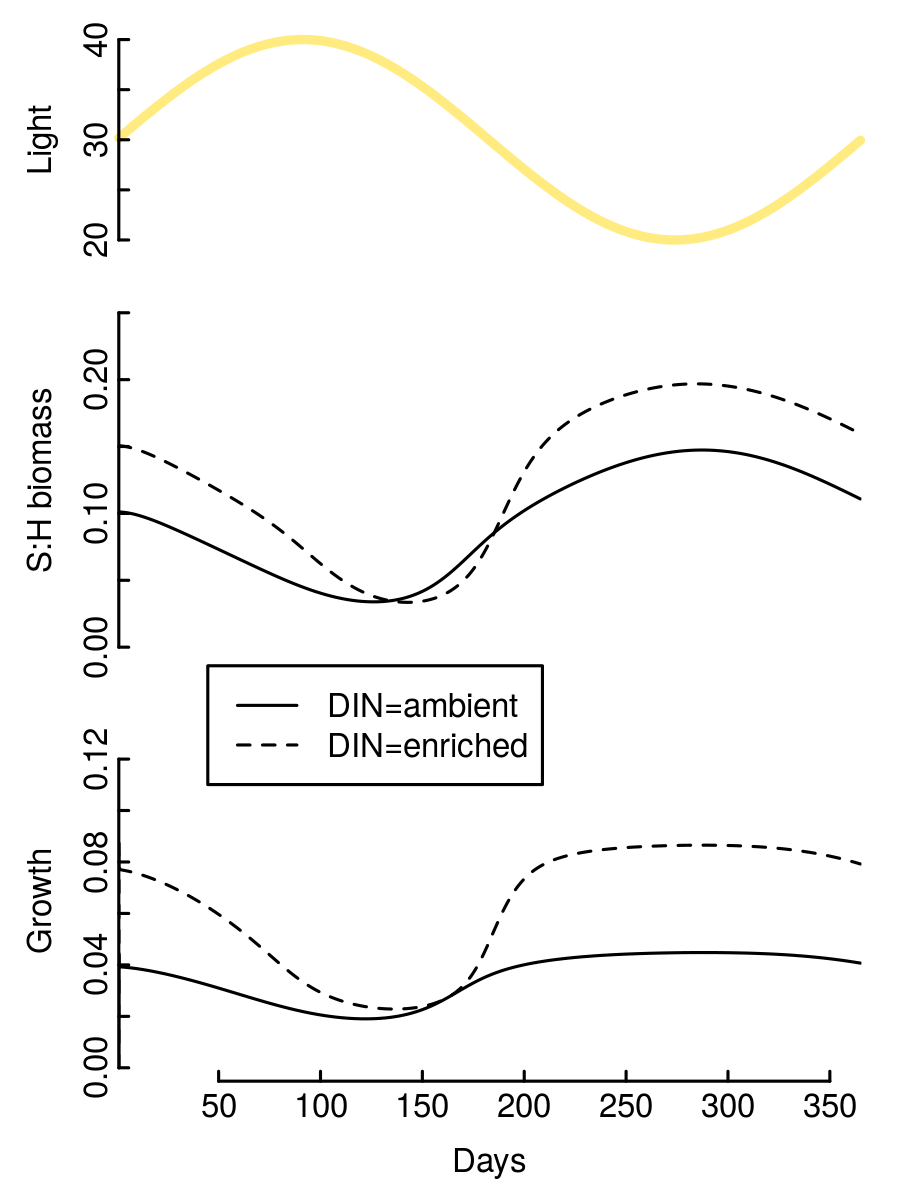
\includegraphics{../img/Fig4.png}
\caption{Sensitivity analysis. Plots show the fractional change in
steady state values of growth (solid lines) and S:H biomass (dashed
lines) in response to fractional changes in default parameter values
(see Table 2 for default values). Parameters are grouped by which
processes they are involved in. This sensitivity analysis was conducted
at conditions typical for coral reef environments: low DIN (1e-7 M) and
intermediate light (15 mol m\textsuperscript{-2} d\textsuperscript{-2}).
Sensitivity analyses conducted other environmental conditions are
presented in Figs S3-S7.}
\end{figure}

Overall, relative changes in the steady state of the system are less
than the equivalent relative change in parameter value, indicating that
the system maintains internal stability. However, changes in certain
parameter values have more significant impacts: increasing \(j_{Nm}\) or
decreasing \(K_N\) both dramatically increase host growth (Fig. 4),
demonstrating the strong nitrogen-limitation that characterizes these
symbioses. The parameter \(\bar{a}^*\) has a strong impact on S:H
biomass ratios (Fig. 4) since this parameter determines the amount of
light absorbed by symbionts, with lower values increasing
light-limitation. Increasing the maximum growth and turnover rates have
the expected effects of increasing and decreasing growth, respectively.
Parameters relating to photooxidative stress and bleaching have little
impact under these environmental conditions (Fig. 4), but have larger
impacts under higher light (e.g., Fig. S6). Sensitivity analyses
conducted under different combinations of external light and nutrients
are presented in Figs. S3-S7.

\section{Dynamic behavior}\label{dynamic-behavior}

The dynamic behavior of the model demonstrates its power to integrate
multiple environmental forcings simultaneously. Here we present several
scenarios that demonstrate the model's ability to reproduce complex
phenomena that have been observed in corals.

\subsection{Seasonal variability}\label{seasonal-variability}

Symbiont densities and coral growth rates are known to vary seasonally,
representing an integrated response to changes in a suite of
environmental factors. Light in particular is a strong driver of these
trends (Stimson 1997; Brown et al. 1999; Fagoonee et al. 1999; Fitt et
al. 2000), with high light associated with lower symbiont abundance and
reduced tissue biomass. The role of light in driving seasonal changes in
symbiont density was demonstrated nicely by Stimson (1997), who also
found that experimental nutrient-enrichment amplified the light-driven
seasonal oscillation. Using the levels of light and nutrients from this
study as inputs, the model reproduces this observed interaction among
environmental factors (Fig. 5), and also provides the mechanism: under
high light in summer, photooxidative stress decreases symbiont biomass
and increases carbon-limitation of host growth regardless of nutrient
status; when light is reduced in winter, growth and symbiont biomass
become constrained instead by nitrogen, and therefore increase more when
DIN is enriched (Fig. S8).

\begin{figure}[htbp]
\centering
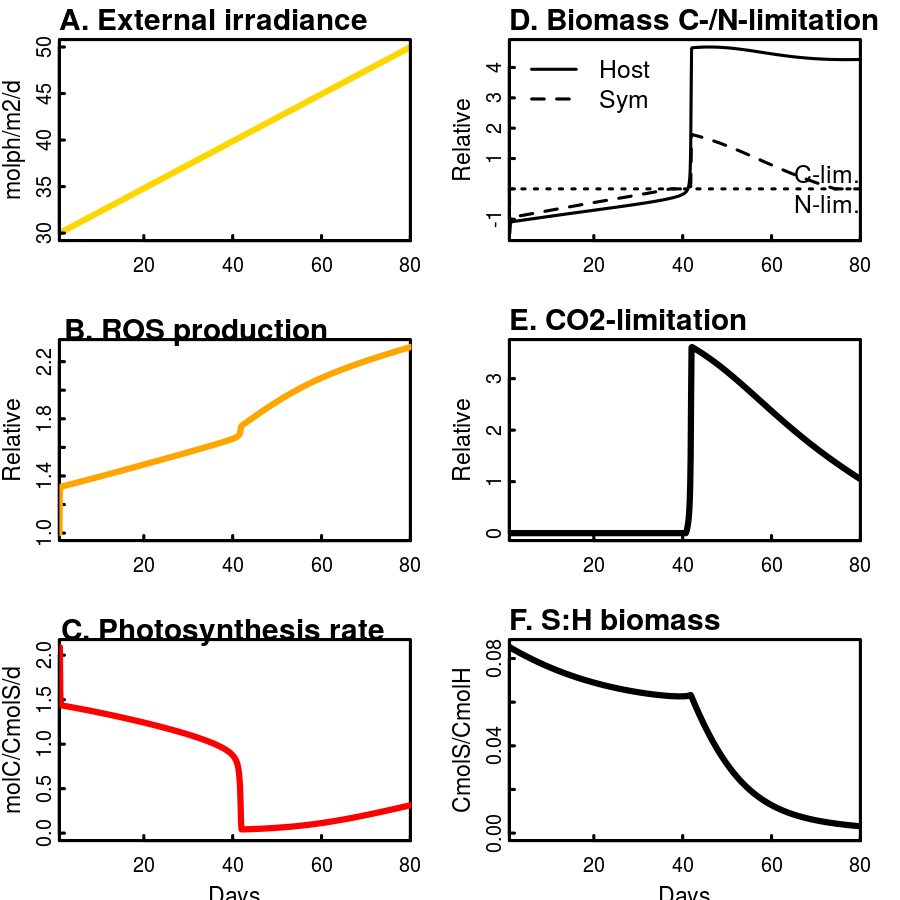
\includegraphics{../img/Fig5.png}
\caption{Light-driven seasonal dynamics of symbiont abundance and coral
growth. Light input (upper panel) was designed as a sinusoidal curve
with a period of one year, with maximum and minimum values of 44 and 22
mol photons m\textsuperscript{-2} d\textsuperscript{-1}, based on
Stimson (1997). The dynamic behavior of symiont to host biomass ratio
(middle panel) and the specific growth rate of host biomass (lower
panel) show seasonal oscillations that are greater in magnitude under
higher nutrients (1e-5 molN L\textsuperscript{-1}; dashed lines)
relative to lower nutrients (1e-7 molN L\textsuperscript{-1}; solid
lines), consistent with the findings of Stimson (1997). Prey density was
set at 1e-5 CmolX L\textsuperscript{-1}.}
\end{figure}

The prediction of higher growth when light is reduced indicates that
growth is not limited by low light in winter, but is actually reduced by
excess light in summer, consistent with the experimental findings of
Schutter et al. (2011). Seasonal summertime reductions in tissue biomass
have also been well-documented in the field (Fitt et al. 2000), along
with reductions in net photosynthetic capacity (Muller-Parker 1987).
Importantly, while light alone (at these levels) may drive seasonal
dynamics in the ways discussed, temperature fluctuations may attenuate
or even reverse the effect of light as cooler winters depress
metabolism; thus, the relative magnitude of fluctuation in temperature,
light, and other factors may produce wide variability in the direction
and magnitude of seasonal changes in growth and symbiont abundance,
depending on location and microhabitat. Nevertheless, the seasonal
variability predicted here (Fig. 5) is consistent with experimental and
field observations for corals, and demonstrates the power of this model
to predict dynamic behavior that mechanistically integrates multiple
environmental drivers.

\subsection{Coral bleaching and
recovery}\label{coral-bleaching-and-recovery}

Coral bleaching is the stress-induced loss of symbiotic algae from coral
tissues, which can occur in response to a variety of environmental
stressors. In most cases, coral bleaching is thought to begin with
photooxidative stress in symbiont photosynthesis (Lesser 1997), which
triggers a cascade of events leading to symbiont expulsion (Weis 2008).
As symbionts are expelled, the host receives less fixed carbon, which
may then compromise its ability to activate CCMs that deliver
CO\textsubscript{2} to photosynthesis (Wooldridge 2013). Increasing
CO\textsubscript{2}-limitation for remaining symbionts, along with an
amplified internal light environment due to reduced self-shading
(Enríquez, Méndez, and Iglesias-Prieto 2005), may further exacerbate
photooxidative stress and accelerate symbiont expulsion, driving the
coral into a bleached state.

While these positive feedbacks have been discussed previously in the
literature, this is the first attempt to implement and explore their
properties within a dynamical model. Interestingly, these feedbacks lead
to alternate stable states in the symbiotic system. The `healthy' state
is characterized by nitrogen-limitation of both symbiont and host: under
these conditions, the symbiont translocates sufficient carbon to support
host growth and CCMs, which ensures that photosynthesis does not become
CO\textsubscript{2}-limited. However, if carbon translocation is
disrupted (and light is sufficiently high), then the system is driven
into the `bleached' state by photooxidative stress and positively
reinforcing carbon- and CO\textsubscript{2}-limitation. In this context,
coral bleaching can be understood as a transition from one stable state
to another, and bleaching thresholds are sets of environmental
conditions that push a healthy-state coral onto a trajectory leading to
a bleached state.

We are highly interested in the conditions under which the system
switches from a healthy to a bleached state, and can use this model as a
tool to explore this dynamic behavior. Most straightforwardly, this
switch occurs when increasing external irradiance (Fig. 6A) causes
sufficient ROS production (Fig. 6B) and photoinhibition (Fig. 6C) such
that the positive feedbacks between host carbon-limitation (Fig. 6D) and
CO\textsubscript{2}-limitation of photosynthesis (Fig. 6E) are rapidly
engaged, leading to even greater photooxidative stress and a rapid
decline in S:H biomass (Fig. 6F), characteristic of coral bleaching.
However, the positive feedbacks involved in bleaching are not engaged
only in response to high external irradiance alone; in fact, they depend
on the relative balance of light energy absorption and quenching, which
in turn depends on the availability of CO\textsubscript{2} for
photosynthesis. While previous models framed photooxidative stress as a
fixed response to absolute external irradiance (Eynaud, Nisbet, and
Muller 2011), our implementation considers the dynamic balance of
multiple energy sinks in the causation of stress, which is more
consistent with current understanding of symbiosis dysfunction
(Wooldridge 2013), and establishes a critical role of host CCMs in
providing CO\textsubscript{2} for photosynthesis (Tansik, Fitt, and
Hopkinson 2015; Hopkinson, Tansik, and Fitt 2015).

\begin{figure}[htbp]
\centering
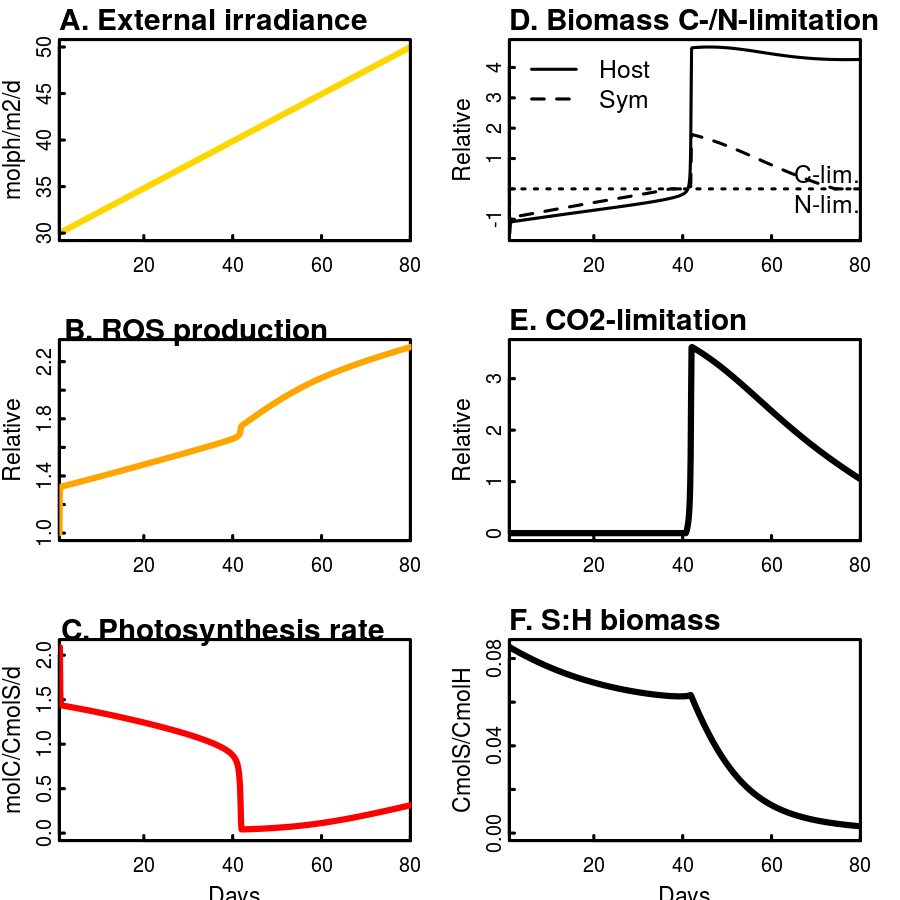
\includegraphics{../img/Fig6.png}
\caption{Coral bleaching as a switch from a nitrogen- to carbon-limited
alternative stable state. This transition is demonstrated in response to
gradually increasing external light (A), which causes an increase in
production of ROS (B) that reduces the photosynthetic rate through
photoinhibition (C). Decreasing photosynthesis moves the system from
overall nitrogen-limitation toward carbon-limitation (D); when this
threshold is crossed, the system rapidly becomes highly carbon-limited
as photosynthesis becomes CO\textsubscript{2}-limited (E) and symbiont
densities rapidly decline (F) into a bleached state. (All parameters at
default values; external DIN=1e-7 molN/L, prey density=0).}
\end{figure}

The importance of host CCM activity establishes significant interactive
roles for other factors in influencing coral bleaching responses. For
example, simulations of high light stress (Fig. 7) demonstrate that
bleaching can be attenuated by heterotrophic feeding, a phenomenon which
has been observed experimentally (Borell et al. 2008). The mechanism
underlying this prediction is that feeding by the host increases host
CCM activity, which delays the onset of CO\textsubscript{2}-limitation
of photosynthesis and reduces bleaching severity. On the other hand,
elevated nutrients exacerbate bleaching (Fig. 7), since higher symbiont
densities are more susceptible to CO\textsubscript{2}-limitation
(Wooldridge 2009). Several experimental (Cunning and Baker 2013; Vega
Thurber et al. 2014) and correlational studies (Wooldridge and Done
2009) are consistent with this mechanistic link between high nutrients
and bleaching.

\begin{figure}[htbp]
\centering
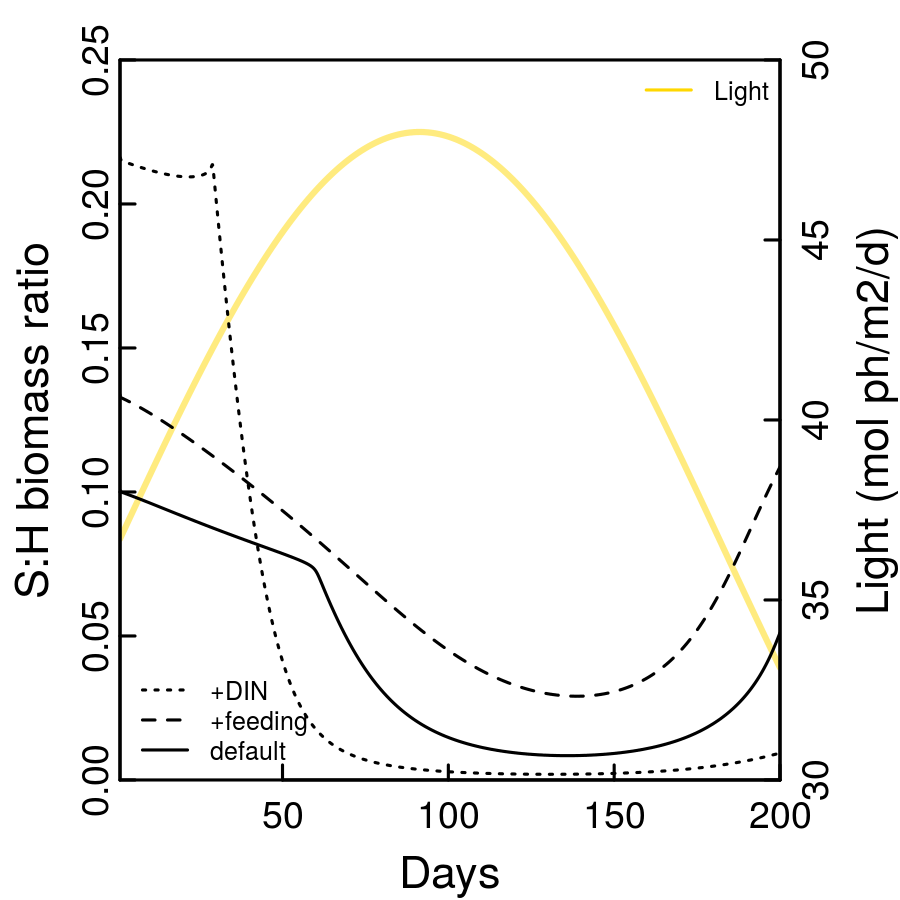
\includegraphics{../img/Fig7.png}
\caption{Bleaching with interactive factors. Simulations of high light
stress (sinusoid with maximum=48 mol ph m\textsuperscript{-2}
d\textsuperscript{-1}) under default environmental conditions (solid
line; DIN=1e-7 molN L\textsuperscript{-1}; prey=3e-6 CmolX
L\textsuperscript{-1}), or with elevated feeding (dashed line; prey=6e-6
CmolX L\textsuperscript{-1}), or elevated nutrients (dotted line;
DIN=1e-6 molN L\textsuperscript{-1}). Initial symbiont biomass was set
to the steady state for each set of starting conditions, respectively.
(All parameters set to default values).}
\end{figure}

Since bleaching is induced by an external stressor, recovery from
bleaching cannot occur unless the stressor is alleviated. In natural
settings, this typically occurs by seasonal declines in temperature and
light. However, alternate stable states lead to significant hysteresis,
indicating that a coral cannot recover along the same trajectory it
followed during bleaching; indeed, the stressor must be alleviated well
\emph{below} the threshold that initially caused bleaching in order for
the system to recover (Fig. 2; Fig. X). This is because under the same
external conditions, a bleached coral (relative to a healthy one) is
characterized by greater light amplification and weaker CCM activity,
which serve to maintain the bleached state. The magnitude of hysteresis
will depend on external nutrients and prey availability, as well as
model parameters, yet the core behavior of hysteresis illustrates the
alternate stable states that exist in the symbiotic system.

\begin{figure}[htbp]
\centering
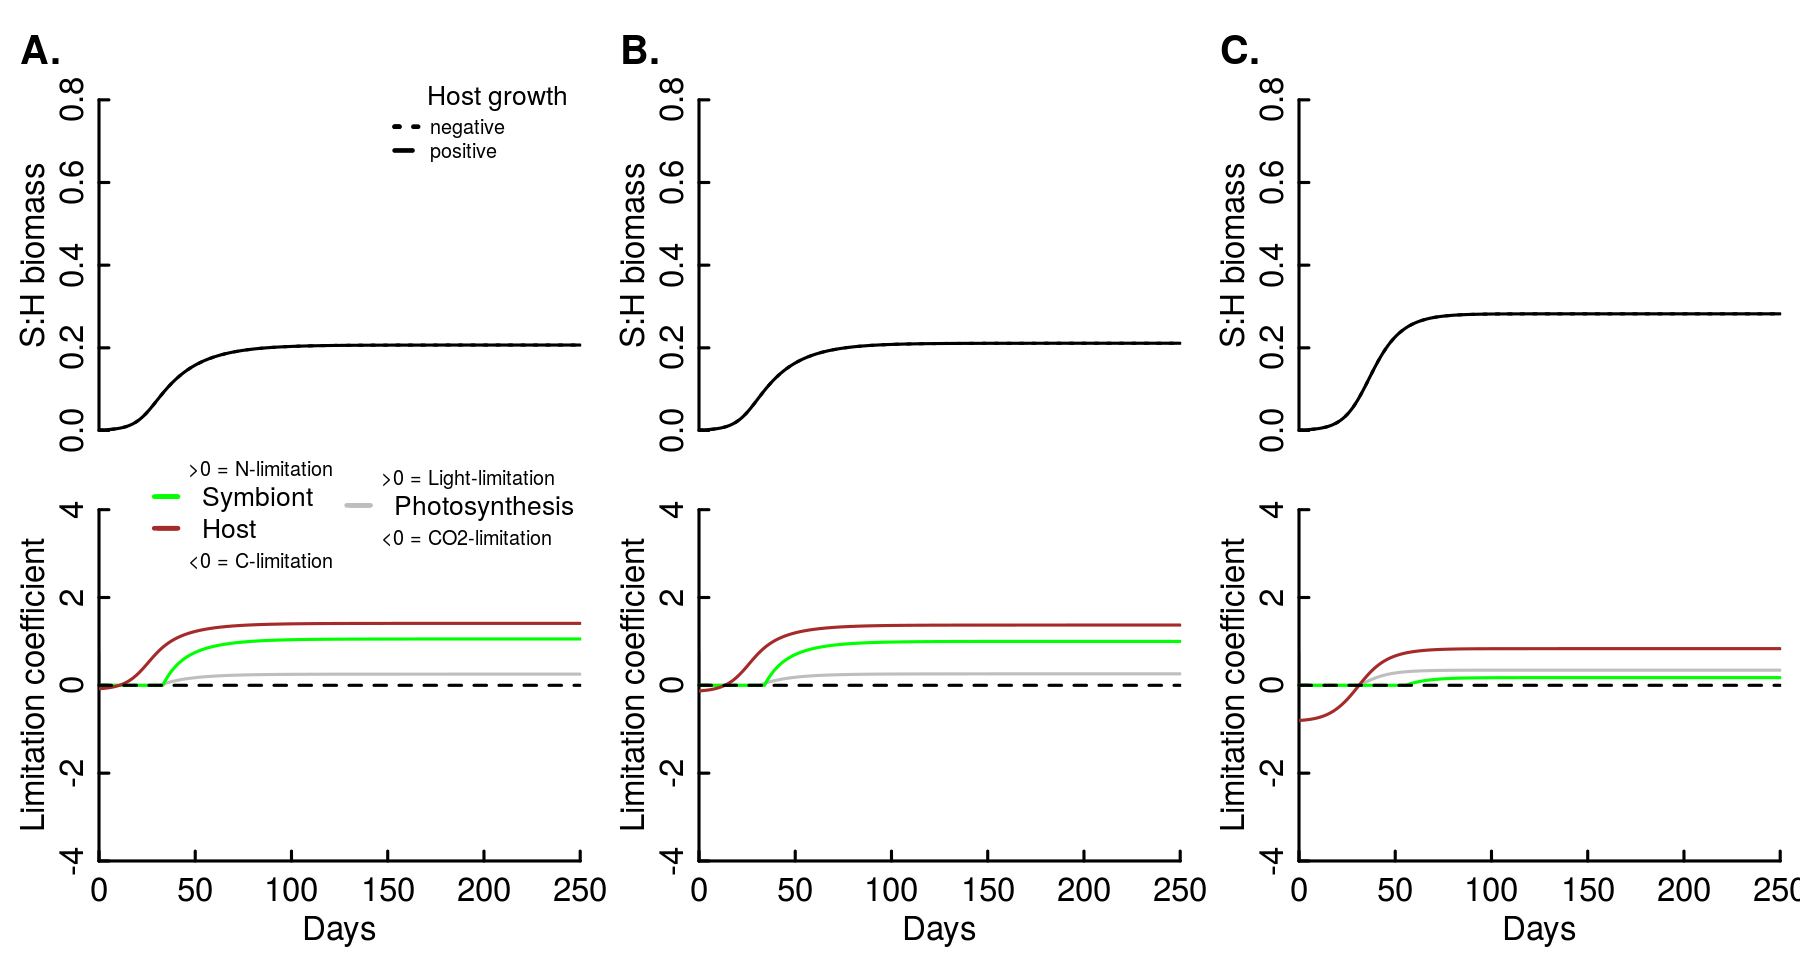
\includegraphics{../img/Fig8.png}
\caption{Recovery from bleaching under varying N:C availability. Higher
N:C ratios in a heterotrophic food source (effectively representing
higher external DIN and/or lower feeding rates) cause a larger overshoot
in the S:H biomass ratio, and prolong the duration of time until the
system `recovers' by re-establishing nitrogen-limitation (represented by
black dots on each trajectory). All simulations run with default
parameters (except varying nNX), L=10 mol photons m\textsuperscript{2}
d\textsuperscript{-1}, DIN=1e-7 molN L\textsuperscript{-1}, prey=1e-6
CmolX L\textsuperscript{-1}, and initial S:H biomass=0.0001.}
\end{figure}

The dynamics of recovery from bleaching reveal another interesting
behavior of the system: under some conditions, the S:H biomass ratio may
increase to a higher value that `overshoots' the ratio maintained in the
`healthy' state under the same conditions (Fig. 8; Fig. S9). In fact,
unusually high symbiont densities have been observed after recovery from
bleaching in both experimental (Cunning, Silverstein, and Baker 2015)
and field studies (Kemp et al. 2014), and have been interpreted as a
potential `disequilibrium in host-symbiont regulation' (Kemp et al.
2014). The model explains this `overshoot' as an approach to a
bifurcation point in the dynamical system \textless{}\textgreater{}. As
the symbiont begins repopulating the host, CO\textsubscript{2} is
limiting and nitrogen is replete, allowing nearly all fixed carbon to be
used for symbiont growth. As a result, host growth remains strongly
carbon-limited, CCM activity remains weak, and photosynthesis remains
CO\textsubscript{2}-limited. As long as this carbon-limitation persists,
S:H biomass will continue to increase beyond the `healthy' steady state
level, until the symbiont population eventually reaches a high enough
density such that nitrogen limits its growth more strongly than carbon.
At this point, which represents the peak of the `overshoot', the
symbiont begins to share carbon with the host, which then supplies more
CO\textsubscript{2} for photosynthesis, etc., causing the system to
rapidly escape the positive feedbacks that were maintaining
carbon-limitation (see Fig. S9 for illustration of all fluxes during
overshoot). The re-establishment of nitrogen-limitation resumes high
rates of carbon fixation and coral growth, bringing the S:H biomass
ratio back down to a stable equilibrium.

The occurrence and the magnitude of this overshoot depend on the
relative inputs of carbon and nitrogen to the system -- any factor that
enhances carbon-limitation (e.g.~high DIN and/or low feeding) therefore
magnifies the overshoot and prolongs the dysfunctional, carbon-limited
state of the symbiosis (Fig. 8). On the other hand, factors that favor
nitrogen-limitation, such as low external DIN and/or high feeding rates,
will accelerate the re-establishment of nitrogen-limitation and prevent
an overshoot from occurring at all. While many scenarios are possible
under different environmental conditions, we illustrate the general
effects of varying N and C availability on recovery from bleaching with
a series of simulations that vary the N:C ratio of host's heterotrophic
food source (Fig. 8): lower N:C ratios (effectively representing lower
DIN and/or higher heterotrophy) favor nitrogen-limitation and more rapid
recovery, while higher N:C ratios (effectively representing higher DIN
and/or lower heterotrophy) favor carbon-limitation and prolonged
recovery with a larger overshoot in S:H biomass.

Importantly, the re-establishment of nitrogen-limitation is the most
important diagnostic of recovery to a `healthy' state, as this is when
high carbon fixation and growth rates are resumed. A high S:H biomass
ratio alone does not indicate that a `healthy' state has been reached,
since overall C-limitation may still persist (e.g., high N:C ratios in
Fig. 8). This could explain why corals that have apparently recovered
their symbiont populations after bleaching still have reduced growth and
reproduction rates until much later (xxx, Hughes). Therefore,
acquisition of carbon from a source other than the symbiont may be
extremely important for the host in order to recover from bleaching.
Indeed, feeding has been shown to promote more rapid recovery from
bleaching (xxx). Moreover, if the host obtains carbon from another
independent source, such as direct uptake of DOC (xxx), this could be
even more important in ensuring rapid recovery from a bleached state.

\section{Conclusions}\label{conclusions}

This simplified dynamic bioenergetic model of coral-\emph{Symbiodinium}
symbioses mechanistically reproduces patterns in steady-state coral
growth and symbiont abundance commonly observed in corals, including
higher symbiont abundance with higher nutrients and feeding, lower
symbiont abundance with increasing light, and optimal growth at
intermediate light levels. Moreover, the model reproduces complex
dynamic behaviors including seasonal changes in symbiont density at
different nutrient levels, rapid bleaching above a threshold of high
light, mitigation of bleaching by heterotrophic feeding, exacerbation of
bleaching by elevated nutrients, and an overshoot of symbiont density
during recovery from bleaching. These examples demonstrate the model's
ability to integrate multiple environmental forcing functions to
reproduce complex responses; meanwhile, the diversity of these phenomena
suggest the model has captured many of the important features of the
system in a unifying mechanistic framework. This model also provides a
new conceptual framework for considering coral bleaching as a transition
to an alternate stable state, which has important implications for
understanding the performance and maintenance of symbiotic interactions.
In this context, the `healthy' stable state represents a scenario in
which the host is `in control' of the system, with nitrogen-limitation
stabilizing the symbiont to host biomass ratio and maintaining positive
growth. Conversely, carbon-limitation represents a loss of host
`control', wherein positive feedbacks result in a loss of capacity for
photosynthetic carbon fixation and positive growth. Importantly, these
`control' mechanisms arise entirely passively through feedbacks present
in the system.

In addition to the suite of specific examples presented here, the model
can be used to explore many different dynamic environmental scenarios,
and represents a tool that biologists and ecologists can use to generate
hypotheses and make predictions in both experimental and natural
settings. Moreover, parameter values can be modified to correspond to
different genetic or functional types of coral hosts and
\emph{Symbiodinium} partners in order to evaluate variability in system
responses. Thus, the diversity of potential applications for this model
is high, and we envision this work as a foundation for continued
development, which may include more detailed treatments of specific
modules (e.g., DIC processing), and the incorporation of more external
forcing capabilities (e.g., external DIC). Importantly, this effort is
best undertaken by the scientific community at large, including those
with theoretical and empirical backgrounds, which is why the code for
this model has been developed openly using the R language. Ultimately,
the continued refinement of these tools is fundamental in elucidating
the mechanisms of symbiosis function and dysfunction, and in predicting
coral responses to environmental change.

\section*{References}\label{references}
\addcontentsline{toc}{section}{References}

\hypertarget{refs}{}
\hypertarget{ref-Anthony:2002tc}{}
Anthony, K. 2002. ``Comparative analysis of energy allocation to tissue
and skeletal growth in corals.'' \emph{Limnology and Oceanography} 47
(5): 1417--29.
\url{https://www.scopus.com/inward/record.uri?partnerID=HzOxMe3b\&scp=0036733455\&origin=inward}.

\hypertarget{ref-ArmozaZvuloni:2014ju}{}
Armoza-Zvuloni, Rachel, Esti Kramarsky-Winter, Yossi Loya, Ami
Schlesinger, and Hanna Rosenfeld. 2014. ``Trioecy, a unique breeding
strategy in the sea anemone Aiptasia diaphana and its association with
sex steroids.'' \emph{Biology of Reproduction} 90 (6). Society for the
Study of Reproduction: 122--22.
doi:\href{https://doi.org/10.1095/biolreprod.113.114116}{10.1095/biolreprod.113.114116}.

\hypertarget{ref-Bak:1976bv}{}
Bak, R. 1976. ``The growth of coral colonies and the importance of
crustose coralline algae and burrowing sponges in relation with
carbonate accumulation.'' \emph{Netherlands Journal of Sea Research} 10
(3): 285--337.
doi:\href{https://doi.org/10.1016/0077-7579(76)90009-0}{10.1016/0077-7579(76)90009-0}.

\hypertarget{ref-Baker:2015kp}{}
Baker, Andrew C, and Ross Cunning. 2015. ``Coral 'Bleaching' as a
Generalized Stress Response to Environmental Disturbance.'' In
\emph{Diseases of Coral}, 396--409. Hoboken, NJ: John Wiley \& Sons,
Inc.
doi:\href{https://doi.org/10.1002/9781118828502.ch30}{10.1002/9781118828502.ch30}.

\hypertarget{ref-Baker:1975ip}{}
Baker, P, and Jon N Weber. 1975. ``Coral growth rate: Variation with
depth.'' \emph{Earth and Planetary Science Letters} 27 (1): 57--61.
doi:\href{https://doi.org/10.1016/0012-821X(75)90160-0}{10.1016/0012-821X(75)90160-0}.

\hypertarget{ref-Barott:2014gx}{}
Barott, Katie L, Alexander A Venn, Sidney O Perez, Sylvie Tambutte, and
Martin Tresguerres. 2014. ``Coral host cells acidify symbiotic algal
microenvironment to promote photosynthesis.'' \emph{Proceedings Of The
National Academy Of Sciences Of The United States Of America}, December.
National Acad Sciences, 201413483.
doi:\href{https://doi.org/10.1073/pnas.1413483112}{10.1073/pnas.1413483112}.

\hypertarget{ref-Borell:2008p108}{}
Borell, Esther M, Ade Yuliantri, Kai Bischof, and Claudio Richter. 2008.
``The effect of heterotrophy on photosynthesis and tissue composition of
two scleractinian corals under elevated temperature.'' \emph{Journal of
Experimental Marine Biology and Ecology} 364: 116--23.

\hypertarget{ref-Brown:1999p3534}{}
Brown, Barbara E, R P Dunne, I Ambarsari, Martin Le Tissier, and U
Satapoomin. 1999. ``Seasonal fluctuations in environmental factors and
variations in symbiotic algae and chlorophyll pigments in four
Indo-Pacific coral species.'' \emph{Marine Ecology Progress Series} 191:
53--69.

\hypertarget{ref-Coles:1978p1124}{}
Coles, SL, and Paul L Jokiel. 1978. ``Synergistic effects of
temperature, salinity and light on the hermatypic coral Montipora
verrucosa.'' \emph{Marine Biology} 49: 187--95.
\url{http://www.springerlink.com/index/LU582837924G7674.pdf}.

\hypertarget{ref-Costanza:2014ex}{}
Costanza, R, R de Groot, and P Sutton. 2014. ``Changes in the global
value of ecosystem services.'' \emph{Global Environmental Change} 26:
152--58.
doi:\href{https://doi.org/10.1016/j.gloenvcha.2014.04.002}{10.1016/j.gloenvcha.2014.04.002}.

\hypertarget{ref-Cunning:2013gp}{}
Cunning, Ross, and Andrew C Baker. 2013. ``Excess algal symbionts
increase the susceptibility of reef corals to bleaching.'' \emph{Nature
Climate Change} 3 (March): 259--62.
doi:\href{https://doi.org/10.1038/nclimate1711}{10.1038/nclimate1711}.

\hypertarget{ref-Cunning:2015ja}{}
Cunning, Ross, Rachel N Silverstein, and Andrew C Baker. 2015.
``Investigating the causes and consequences of symbiont shuffling in a
multi-partner reef coral symbiosis under environmental change.''
\emph{Proceedings of the Royal Society B}, 1--9.
doi:\href{https://doi.org/10.1098/rspb.2014.1725\%7B/\&\%7Ddomain=pdf\%7B/\&\%7Ddate_stamp}{10.1098/rspb.2014.1725\{\textbackslash{}\&\}domain=pdf\{\textbackslash{}\&\}date\_stamp}.

\hypertarget{ref-Downs:2013kc}{}
Downs, C A, Kathleen E McDougall, Cheryl M Woodley, John E Fauth, Robert
H Richmond, Ariel Kushmaro, Stuart W Gibb, Yossi Loya, Gary K Ostrander,
and Esti Kramarsky-Winter. 2013. ``Heat-Stress and Light-Stress Induce
Different Cellular Pathologies in the Symbiotic Dinoflagellate during
Coral Bleaching.'' \emph{PLoS ONE} 8 (12): e77173.
doi:\href{https://doi.org/10.1371/journal.pone.0077173}{10.1371/journal.pone.0077173}.

\hypertarget{ref-Edmunds:2011bv}{}
Edmunds, Peter J, Hollie M Putnam, Roger M Nisbet, and Erik B Muller.
2011. ``Benchmarks in organism performance and their use in comparative
analyses.'' \emph{Oecologia} 167 (2): 379--90.
doi:\href{https://doi.org/10.1007/s00442-011-2004-2}{10.1007/s00442-011-2004-2}.

\hypertarget{ref-Enriquez:2005p142}{}
Enríquez, Susana, Eugenio R Méndez, and Roberto Iglesias-Prieto. 2005.
``Multiple scattering on coral skeletons enhances light absorption by
symbiotic algae.'' \emph{Limnology and Oceanography} 50 (4): 1025--32.

\hypertarget{ref-Eynaud:2011tv}{}
Eynaud, Yoan, Roger M Nisbet, and Erik B Muller. 2011. ``Impact of
excess and harmful radiation on energy budgets in scleractinian
corals.'' \emph{Ecological Modelling} 222 (7). Elsevier: 1315--22.
\url{http://www.sciencedirect.com/science/article/pii/S0304380011000263}.

\hypertarget{ref-Fagoonee:1999p4136}{}
Fagoonee, I, H B Wilson, M P Hassell, and J R Turner. 1999. ``The
Dynamics of Zooxanthellae Populations: A Long-Term Study in the Field.''
\emph{Science} 283 (5403): 843--45.
doi:\href{https://doi.org/10.1126/science.283.5403.843}{10.1126/science.283.5403.843}.

\hypertarget{ref-FerrierPages:2000p1950}{}
Ferrier-Pagès, Christine, Jean-Pierre Gattuso, S Dallot, and Jean
Jaubert. 2000. ``Effect of nutrient enrichment on growth and
photosynthesis of the zooxanthellate coral Stylophora \ldots{}.''
\emph{Coral Reefs}.
\url{http://www.springerlink.com/index/3DRC3K1Q57TPC0UT.pdf}.

\hypertarget{ref-Fitt:2000p3792}{}
Fitt, William K, F K McFarland, Mark E Warner, and Geoff C Chilcoat.
2000. ``Seasonal patterns of tissue biomass and densities of symbiotic
dinoflagellates in reef corals and relation to coral bleaching.''
\emph{Limnology and Oceanography} 45 (3): 677--85.

\hypertarget{ref-Hawkins:2016jj}{}
Hawkins, Thomas D, Julia C G Hagemeyer, Kenneth D Hoadley, Adam G Marsh,
and Mark E Warner. 2016. ``Partitioning of Respiration in an
Animal-Algal Symbiosis: Implications for Different Aerobic Capacity
between Symbiodinium spp.'' \emph{Frontiers in Physiology} 7 (April).
Frontiers: 125.
doi:\href{https://doi.org/10.3389/fphys.2016.00128}{10.3389/fphys.2016.00128}.

\hypertarget{ref-HoeghGuldberg:1999p4222}{}
Hoegh-Guldberg, Ove. 1999. ``Climate change, coral bleaching and the
future of the world's coral reefs.'' \emph{Marine and Freshwater
Research} 50 (November): 839--66.

\hypertarget{ref-Hopkinson:2015ev}{}
Hopkinson, Brian M, Anna L Tansik, and William K Fitt. 2015. ``Internal
carbonic anhydrase activity in the tissue of scleractinian corals is
sufficient to support proposed roles in photosynthesis and
calcification.'' \emph{The Journal of Experimental Biology}, April. The
Company of Biologists Ltd, jeb.118182.
doi:\href{https://doi.org/10.1242/jeb.118182}{10.1242/jeb.118182}.

\hypertarget{ref-Huston:1985ec}{}
Huston, M. 1985. ``Variation in coral growth rates with depth at
Discovery Bay, Jamaica.'' \emph{Coral Reefs} 4 (1): 19--25.
doi:\href{https://doi.org/10.1007/BF00302200}{10.1007/BF00302200}.

\hypertarget{ref-Jager:2013bj}{}
Jager, Tjalling, Benjamin T Martin, and Elke I Zimmer. 2013. ``DEBkiss
or the quest for the simplest generic model of animal life history.''
\emph{Journal of Theoretical Biology} 328: 9--18.
doi:\href{https://doi.org/10.1016/j.jtbi.2013.03.011}{10.1016/j.jtbi.2013.03.011}.

\hypertarget{ref-Jokiel:1977p7353}{}
Jokiel, Paul L, and SL Coles. 1977. ``Effects of temperature on the
mortality and growth of Hawaiian reef corals.'' \emph{Marine Biology} 43
(3): 201--8.

\hypertarget{ref-Jones:1998p3572}{}
Jones, Ross J, Ove Hoegh-Guldberg, Anthony W D Larkum, and Ulrich
Schreiber. 1998. ``Temperature-induced bleaching of corals begins with
impairment of the CO2 fixation mechanism in zooxanthellae.''
\emph{Plant, Cell and Environment} 21 (12): 1219--30.

\hypertarget{ref-Kemp:2014ug}{}
Kemp, Dustin W, X Hernandez-Pech, Roberto Iglesias-Prieto, William K
Fitt, and Gregory W Schmidt. 2014. ``Community dynamics and physiology
of Symbiodinium spp. before, during, and after a coral bleaching
event.'' \emph{Limnology and Oceanography}.
\url{http://www.aslo.org/lo/pdf/vol_59/issue_3/0788.pdf}.

\hypertarget{ref-Kooijman:2010vd}{}
Kooijman, SALM. 2010. \emph{Dynamic Energy Budget Theory for Metabolic
Organization}. 3rd ed. Cambridge University Press.

\hypertarget{ref-Lesser:1997p3587}{}
Lesser, Michael P. 1997. ``Oxidative stress causes coral bleaching
during exposure to elevated temperatures.'' \emph{Coral Reefs} 16
(July): 187--92.

\hypertarget{ref-Marcelino:2013hz}{}
Marcelino, Luisa A, Mark W Westneat, Valentina Stoyneva, Jillian Henss,
Jeremy D Rogers, Andrew Radosevich, Vladimir Turzhitsky, et al. 2013.
``Modulation of Light-Enhancement to Symbiotic Algae by Light-Scattering
in Corals and Evolutionary Trends in Bleaching.'' \emph{PLoS ONE} 8 (4):
e61492.
doi:\href{https://doi.org/10.1371/journal.pone.0061492.s008}{10.1371/journal.pone.0061492.s008}.

\hypertarget{ref-Marubini:1996p8460}{}
Marubini, F, and PS Davies. 1996. ``Nitrate increases zooxanthellae
population density and reduces skeletogenesis in corals.'' \emph{Marine
Biology} 127 (2): 319--28.
\url{http://www.scopus.com/inward/record.url?partnerID=yv4JPVwI\&eid=2-s2.0-0030301761\&md5=0971551a6865f30046294b9e17fb4081}.

\hypertarget{ref-Muller:2009io}{}
Muller, Erik B, Sebastiaan A L M Kooijman, Peter J Edmunds, Francis J
Doyle, and Roger M Nisbet. 2009. ``Dynamic energy budgets in syntrophic
symbiotic relationships between heterotrophic hosts and photoautotrophic
symbionts.'' \emph{Journal of Theoretical Biology} 259 (1): 44--57.
doi:\href{https://doi.org/10.1016/j.jtbi.2009.03.004}{10.1016/j.jtbi.2009.03.004}.

\hypertarget{ref-MullerParker:1987cr}{}
Muller-Parker, Gisèle. 1987. ``Seasonal variation in light-shade
adaptation of natural populations of the symbiotic sea anemone
Aiptasiapulchella (Carlgren, 1943) in Hawaii.'' \emph{Journal of
Experimental Marine Biology and Ecology} 112 (2): 165--83.
doi:\href{https://doi.org/10.1016/0022-0981(87)90115-8}{10.1016/0022-0981(87)90115-8}.

\hypertarget{ref-MullerParker:1994uo}{}
Muller-Parker, Gisèle, Lawrence R McCloskey, Ove Hoegh-Guldberg, and PJ
McAuley. 1994. ``Effect of ammonium enrichment on animal and algal
biomass of the coral Pocillopora damicornis.'' \emph{Pacific Science} 48
(3). \url{http://scholarspace.manoa.hawaii.edu/handle/10125/2236}.

\hypertarget{ref-Muscatine:1977p4220}{}
Muscatine, Leonard, and James W Porter. 1977. ``Reef corals: mutualistic
symbioses adapted to nutrient-poor environments.'' \emph{Bioscience} 27
(7): 454--60.

\hypertarget{ref-Muscatine:1981jy}{}
Muscatine, Leonard, L R McCloskey, and R E Marian. 1981. ``Estimating
the daily contribution of carbon from zooxanthellae to coral animal
respiration.'' \emph{Limnology and Oceanography} 26 (4): 601--11.
doi:\href{https://doi.org/10.4319/lo.1981.26.4.0601}{10.4319/lo.1981.26.4.0601}.

\hypertarget{ref-Osinga:2011kq}{}
Osinga, Ronald, Miriam Schutter, Ben Griffioen, René H Wijffels, Johan A
J Verreth, Shai Shafir, Stéphane Henard, Maura Taruffi, Claudia Gili,
and Silvia Lavorano. 2011. ``The Biology and Economics of Coral
Growth.'' \emph{Marine Biotechnology} 13 (4): 658--71.
doi:\href{https://doi.org/10.1007/s10126-011-9382-7}{10.1007/s10126-011-9382-7}.

\hypertarget{ref-Osinga:2012is}{}
Osinga, Ronald, Miriam Schutter, Tim Wijgerde, Buki Rinkevich, Shai
Shafir, Muki Shpigel, Gian Marco Luna, et al. 2012. ``The CORALZOO
project: a synopsis of four years of public aquarium science.''
\emph{Journal of the Marine Biological Association of the UK} 92 (04).
Cambridge University Press: 753--68.
doi:\href{https://doi.org/10.1017/S0025315411001779}{10.1017/S0025315411001779}.

\hypertarget{ref-Powles:1984tm}{}
Powles, Stephen B. 1984. ``Photoinhibition of photosynthesis induced by
visible light.'' \emph{Annual Review of Plant Physiology} 35: 15--44.

\hypertarget{ref-RALanguageandEn:2014wf}{}
R Core Team. 2014. ``R: A Language and Environment for Statistical
Computing.'' Vienna, Austria: R Foundation for Statistical Computing.
\url{http://www.R-project.org/}.

\hypertarget{ref-Roth:2014wf}{}
Roth, M S. 2014. ``The engine of the reef: Photobiology of the
coral-algal symbiosis.'' \emph{Frontiers in Microbiology}.
\url{http://journal.frontiersin.org/Journal/10.3389/fmicb.2014.00422/pdf}.

\hypertarget{ref-Schutter:2010p7758}{}
Schutter, M, J Crocker, A Paijmans, M Janse, R Osinga, A J Verreth, and
R H Wijffels. 2010. ``The effect of different flow regimes on the growth
and metabolic rates of the scleractinian coral Galaxea fascicularis.''
\emph{Coral Reefs}, April.
doi:\href{https://doi.org/10.1007/s00338-010-0617-2}{10.1007/s00338-010-0617-2}.

\hypertarget{ref-Schutter:2011ie}{}
Schutter, Miriam, Rosa M van der Ven, Max Janse, Johan A J Verreth, René
H Wijffels, and Ronald Osinga. 2011. ``Light intensity, photoperiod
duration, daily light flux and coral growth of Galaxea fascicularis in
an aquarium setting: a matter of photons?'' \emph{Journal of the Marine
Biological Association of the UK} 92 (04). Cambridge University Press:
703--12.
doi:\href{https://doi.org/10.1017/S0025315411000920}{10.1017/S0025315411000920}.

\hypertarget{ref-Shantz:2015dz}{}
Shantz, Andrew A, Nathan P Lemoine, and Deron E Burkepile. 2015.
``Nutrient loading alters the performance of key nutrient exchange
mutualisms.'' \emph{Ecology Letters} 19 (1): 20--28.
doi:\href{https://doi.org/10.1111/ele.12538}{10.1111/ele.12538}.

\hypertarget{ref-Stimson:1997p3837}{}
Stimson, J. 1997. ``The annual cycle of density of zooxanthellae in the
tissues of field and laboratory-held Pocillopora damicornis
(Linnaeus).'' \emph{Journal of Experimental Marine Biology and Ecology}
214 (1-2): 35--48.

\hypertarget{ref-Tanaka:2013dj}{}
Tanaka, Yasuaki, Akira Iguchi, Mayuri Inoue, Chiharu Mori, K Sakai,
Atsushi Suzuki, Hodaka Kawahata, and Takashi Nakamura. 2013. ``Marine
Pollution Bulletin.'' \emph{Marine Pollution Bulletin} 68 (1-2): 93--98.
doi:\href{https://doi.org/10.1016/j.marpolbul.2012.12.017}{10.1016/j.marpolbul.2012.12.017}.

\hypertarget{ref-Tanaka:2007uv}{}
Tanaka, Yasuaki, Toshihiro Miyajima, Isao Koike, Takeshi Hayashibara,
and Hiroshi Ogawa. 2007. ``Imbalanced coral growth between organic
tissue and carbonate skeleton caused by nutrient enrichment.''
\emph{Limnology and Oceanography}.
\url{http://www.aslo.org/lo/toc/vol_52/issue_3/1139.pdf}.

\hypertarget{ref-Tansik:2015cm}{}
Tansik, Anna L, William K Fitt, and Brian M Hopkinson. 2015. ``External
carbonic anhydrase in three Caribbean corals: quantification of activity
and role in CO2 uptake.'' \emph{Coral Reefs} 34 (3). Springer Berlin
Heidelberg: 703--13.
doi:\href{https://doi.org/10.1007/s00338-015-1289-8}{10.1007/s00338-015-1289-8}.

\hypertarget{ref-Titlyanov:2001p3631}{}
Titlyanov, E A, T V Titlyanova, K Yamazato, and Robert van Woesik. 2001.
``Photo-acclimation dynamics of the coral Stylophora pistillata to low
and extremely low light.'' \emph{Journal of Experimental Marine Biology
and Ecology} 263 (2): 211--25.

\hypertarget{ref-VegaThurber:2014hk}{}
Vega Thurber, Rebecca L, Deron E Burkepile, Corinne Fuchs, Andrew A
Shantz, Ryan McMinds, and Jesse R Zaneveld. 2014. ``Chronic nutrient
enrichment increases prevalence and severity of coral disease and
bleaching.'' \emph{Global Change Biology} 20 (2): 544--54.
doi:\href{https://doi.org/10.1111/gcb.12450}{10.1111/gcb.12450}.

\hypertarget{ref-Wang:1998p128}{}
Wang, J, and Angela E Douglas. 1998. ``Nitrogen recycling or nitrogen
conservation in an alga-invertebrate symbiosis?'' \emph{The Journal of
Experimental Biology} 201: 2445--53.

\hypertarget{ref-Warner:1999p4239}{}
Warner, Mark E, William K Fitt, and Gregory W Schmidt. 1999. ``Damage to
photosystem II in symbiotic dinoflagellates: A determinant of coral
bleaching.'' \emph{Proceedings Of The National Academy Of Sciences Of
The United States Of America} 96 (14): 8007--12.

\hypertarget{ref-Weis:2008p944}{}
Weis, Virginia M. 2008. ``Cellular mechanisms of Cnidarian bleaching:
stress causes the collapse of symbiosis.'' \emph{The Journal of
Experimental Biology} 211 (Pt 19): 3059--66.
doi:\href{https://doi.org/10.1242/jeb.009597}{10.1242/jeb.009597}.

\hypertarget{ref-Wooldridge:2009p7807}{}
Wooldridge, Scott A. 2009. ``A new conceptual model for the warm-water
breakdown of the coral-algae endosymbiosis.'' \emph{Marine and
Freshwater Research} 60 (June): 483--96.

\hypertarget{ref-Wooldridge:2010p7809}{}
---------. 2010. ``Is the coral-algae symbiosis really 'mutually
beneficial' for the partners?'' \emph{BioEssays}, May.

\hypertarget{ref-Wooldridge:2013tj}{}
---------. 2013. ``Breakdown of the coral-algae symbiosis: towards
formalising a linkage between warm-water bleaching thresholds and the
growth rate of the intracellular zooxanthellae.'' \emph{Biogeosciences}
10: 1647--58.
\url{http://www.biogeosciences.net/10/1647/2013/bg-10-1647-2013.html}.

\hypertarget{ref-Wooldridge:2014di}{}
---------. 2014a. ``Differential thermal bleaching susceptibilities
amongst coral taxa: re-posing the role of the host.'' \emph{Coral Reefs}
33 (1). Springer Berlin Heidelberg: 15--27.
doi:\href{https://doi.org/10.1007/s00338-013-1111-4}{10.1007/s00338-013-1111-4}.

\hypertarget{ref-Wooldridge:2014hc}{}
---------. 2014b. ``Formalising a mechanistic linkage between
heterotrophic feeding and thermal bleaching resistance.'' \emph{Coral
Reefs}. Springer Berlin Heidelberg, 1--6.
doi:\href{https://doi.org/10.1007/s00338-014-1193-7}{10.1007/s00338-014-1193-7}.

\hypertarget{ref-Wooldridge:2009kb}{}
Wooldridge, Scott A, and Terry J Done. 2009. ``Improved water quality
can ameliorate effects of climate change on corals.'' \emph{Ecological
Applications} 19 (6). Ecological Society of America: 1492--9.
doi:\href{https://doi.org/10.1890/08-0963.1}{10.1890/08-0963.1}.

\hypertarget{ref-Yellowlees:2008p331}{}
Yellowlees, David, T A V Rees, and William Leggat. 2008. ``Metabolic
interactions between algal symbionts and invertebrate hosts.''
\emph{Plant, Cell and Environment} 31: 679--94.

\end{document}


